\documentclass[a4paper,11pt]{article}
\usepackage{physics}
\usepackage{amsmath}
\numberwithin{equation}{section}
\usepackage{siunitx}
\usepackage{braket}
\usepackage{authblk}
\usepackage[a4paper, margin=1.5in]{geometry}
\usepackage{parskip}
\setlength{\parindent}{15pt}
\usepackage{tikz}
\usetikzlibrary{arrows, calc, patterns, angles, quotes}
\usetikzlibrary{decorations.pathmorphing}
\usepackage{amssymb}
\usetikzlibrary{shapes.geometric}
\usepackage[section]{placeins}
\usepackage{pgfplots}
\usepackage{clock}
\usepackage[clock]{ifsym}
\usetikzlibrary{shapes}
%\usepgfplotslibrary{external}
%\tikzexternalize

\begin{document}
\begin{titlepage}\centering
 \clearpage
 \title{\textsc{\bf{SPECIAL RELATIVITY}}\\\smallskip A Quick Guide\\}
 \author{\bigskip Huan Q. Bui}
 \affil{Colby College\\$\,$\\ PHYSICS \& MATHEMATICS\\ Statistics \\$\,$\\Class of 2021\\}
 \date{\today}
 \maketitle
 \thispagestyle{empty}
\end{titlepage}

%
% \noindent \textbf{\huge {Preface}}
 
% \noindent \textit{Introduction to Special Relativity: An Undergraduate's Quick Guide} isn't a textbook, but rather an introduction to Einstein's special relativity which may suit best for the enthusiastic who have had some grasp of the basic ideas of special relativity but wanted something more ``mathy'' to better solidify their understanding of the theory. As suggested, this guide contains mostly of mathematical descriptions, derivations, and consequences of important concepts in special relativity, but with less emphasis on (but by no means absolute exclusion of) historical backgrounds and intuitive explanations. Readers who are eager to enhance their general mathematical mastery of special relativity or are looking for an ``equation handbook'' may find this text helpful. There will be a few sample problems (with readily followed solutions); however, exercises are not immediately relevant to the purpose of this guide, which is to provide readers with a quick walk-through of the concepts of special relativity and its consequences. To truly master special relativity (or any discipline for that matter), readers are encouraged to seek out challenging problem sets and advanced readings on this subject. David J. Morin's \textit{Special Relativity: For the Enthusiastic Beginner} should offer a fantastic start.\\
 
% \noindent \textbf{\huge {A word from me}}
 
% \noindent I am an undergraduate pursuing a Bachelor of Arts (2021) in Physics and Statistics at Colby College, Waterville, Maine, U.S.A. The content of this guide based on my lecture notes from PH241: Modern Physics I, which I took in my first semester of college with professor Charles Conover. This guide is written in my attempt to learn \LaTeX.
% 
% \noindent Enjoy!
% \newpage
%
 
 \tableofcontents
 \newpage
 
 \section{Galilean and Newtonian Relativity}
 \subsection{Two central problems of relativity}
 Two observers in different inertial reference frames $S$ and $S'$ make detailed observations as physical phenomena occur. Each observer records the Time and Location of a set of events. How do their records compare?
 \subsection{Terms defined}
 \subsubsection{Events}
 Something that occurs independent of our description of it (time and location).
 \subsubsection{Observers}
 Someone who compiles measurements of where and when Events occur. Note that measurements of when and where events occur are NOT when and where the observer ``sees'' the events.
 \subsubsection{Inertial reference frame}
 Coordinate systems in which the law of inertia is true.
  \begin{figure}[h!] %place figure here
  \centering
    \begin{tikzpicture}[->, thick]
            \draw (0,0,0) -- (0,3,0) node[above] {$+y$}; %+Y
            \draw (5,0,0) -- (5,3,0) node[above] {$+y'$}; %+y'
            \draw (0,0,0) -- (8,0,0) node[right] {$+x$}; %+x
            \draw (0,0,0) -- (0,0,3.5) node[left] {$+z$}; %z
            \draw (5,0,0) -- (5,0,3.5) node[left] {$+z'$}; %z'
            \draw [->, ultra thick] (6,1.5,0) -- (7,1.5,0) node[right] {\textbf{$\vec{v}$}};
            \node[label={left: \large ${(S)}$}] at (0,1.80,0){};
            \node[label={left: \large ${(S')}$}] at (5,1.80,0){};
    \end{tikzpicture}
    \caption{Frame $(S')$ moves with speed $\vec{v}$ relative to frame $(S)$}
    \label{fig: s to s'}
  \end{figure}
  
 \subsection{Principle of Relativity}
 The laws of physics are the same in \underline{all} inertial reference frames.
 \subsection{Coordinate Transformations}
 If an ``event'' is observed in space-time ordinates $(t,x,y,z)$ in $S$, how do we determine space-time coordinate $(t', x', y', z')$ in $S'$?
 \subsubsection{Spatial Rotation}
  \begin{figure}[h!]
  \centering
   \begin{tikzpicture}[->]
	\draw [->] (0,0,0) -- (0,7,0) node[above] {$y$};
	\draw [->] (0,0,0) -- (7,0,0) node[right] {$x$};
	\draw [dashed] (0,0,0) -- (6.75,1.5,0) node[above] {$x'$};
	\draw [dashed] (0,0,0) -- (-1.5,6.75,0) node[above] {$y'$};
	\draw [->, ultra thick] (0,0,0) -- (6,6,0) node[above] {\large $\vec{r_{p}}$};
	
	\node at (2.3,0.25) {$\theta$};
	\node at (-0.25,2.3) {$\theta$};
	
   \end{tikzpicture}
   \caption{Spatial rotation: $(S)$ being transformed into $(S')$}
   \label{fig: rotate}
  \end{figure}
  
  \begin{equation} \label{eq:1}
  \begin{cases} 
    (S): \vec{r_{p}} = \braket{x_{p}, y_{p}} = x_{p}\hat{i} + y_{p}\hat{j} \\
    (S'): \vec{r_{p}} = \braket{x'_{p}, y'_{p}} = x'_{p}\hat{i'} + y'_{p}\hat{j'}
  \end{cases}
  \end{equation}
  
  \noindent For vector $\vec{r_{p}}$ in our case:
  \begin{equation} \label{eq:2}
   \vec{r_{p}} = x_{p}\hat{i} + y_{p}\hat{j} = x'_{p}\hat{i'} + y'_{p}\hat{j'}
  \end{equation}
  
  \noindent So, for any vector $\vec{a}$:
  \begin{equation} \label{eq:3}
   \vec{r_{a}} = x_{a}\hat{i} + y_{a}\hat{j} = x'_{a}\hat{i'} + y'_{a}\hat{j'}
  \end{equation}
  
  \noindent Unit vectors:
  \begin{equation} \label{eq:4}
  \begin{cases} 
    \hat{i'} = \hat{i} \cos\theta + \hat{j} \sin\theta \\
    \hat{j'} = -\hat{i} \sin\theta + \hat{j} \cos\theta
  \end{cases}
  \end{equation}
  
  \noindent Reversing the transformation:
  \begin{equation} \label{eq:5}
  \begin{cases} 
    \hat{i} = \hat{i'} \cos(-\theta) + \hat{j'} \sin(-\theta) \\
    \hat{j} = -\hat{i'} \sin(-\theta) + \hat{j'} \cos(-\theta)
  \end{cases}
  \end{equation}

  \noindent We can thus find the coefficients $x_{a}$ and $y_{a}$ by combining \eqref{eq:3}, \eqref{eq:4}, and \eqref{eq:5}:\
  \begin{equation} \label{eq:6}
    \begin{split}
      \vec{r_{a}} &= x_{a}\hat{i} + y_{a}\hat{j} \\
      &= x_{a}(\hat{i'} \cos(-\theta) + \hat{j'} \sin(-\theta)) + y_{a}(-\hat{i'} \sin(-\theta) + \hat{j'} \cos(-\theta)) \\
      &= x_{a}(\hat{i'} \cos\theta - \hat{j'} \sin\theta) + y_{a}(\hat{i'} \sin\theta + \hat{j'} \cos\theta) \\
      &= (x_{a}\cos\theta + y_{a}\sin\theta)\hat{i'} + (-x_{a}\sin\theta + y_{a}\cos\theta)\hat{j'} \\
      &= x'_{a}\hat{i'} + y'_{a}\hat{j'}
    \end{split}
  \end{equation}
 
  \noindent Hence, we get: 
  \begin{equation} \label{eq:7}
  \begin{cases} 
    x'_{a} = x_{a}\cos\theta + y_{a}\sin\theta \\ 
    y'_{a} = -x_{a}\sin\theta + y_{a}\cos\theta
  \end{cases}
  \end{equation}
  
  \noindent We can now calculate the magnitude of vector $\vec{a}$ in both frames $(S')$ and $(S')$:
  \begin{equation} \label{eq:8}
    \begin{split}
      (S): ||\vec{a}|| &= {x_{a}}^2 + {y_{a}}^2 \\ 
      (S'): ||\vec{a}|| &= {x^{\prime}_{a}}^2 + {y^{\prime}_{a}}^2 \\
      &= {(x_{a}\cos\theta + y_{a}\sin\theta)}^{2} + {(-x_{a}\sin\theta + y_{a}\cos\theta)}^{2} \\ 
      &= ... \\
      &= ((\cos\theta)^2 + (\sin\theta)^2)({x_{a}}^2 + {y_{a}}^2)\\
      &= {x_{a}}^2 + {y_{a}}^2
    \end{split}
  \end{equation}
  
  \noindent So, different observers would agree on the magnitude of vector $\vec{a}$. We say the magnitude of vector $\vec{a}$ is \textit{invariant} under orthogonal transformations. 
 
 \subsubsection{Galilean Transformation}
 Say, we have two frames $(S)$ and $(S')$. Frame $(S')$ is moving with velocity $\vec{v}$ relative to frame $(S)$. At time $t=t'=0$, $x=x'=0$, $y=y'=0$, and $z=z'=0$. 
 \begin{figure}[!hbt] %place figure here
  \centering
    \begin{tikzpicture}[->, thick]
            \draw (0,0,0) -- (0,2,0) node[above] {$+y$}; %+Y
            \draw (5,0,0) -- (5,2,0) node[above] {$+y'$}; %+y'
            \draw (0,0,0) -- (8,0,0) node[right] {$+x$}; %+x
            \draw (0,0,0) -- (0,0,3.5) node[left] {$+z$}; %z
            \draw (5,0,0) -- (5,0,3.5) node[left] {$+z'$}; %z'
            \draw [->, ultra thick] (6,1.5,0) -- (7,1.5,0) node[right] {\textbf{$\vec{v}$}};
            \node[label={left: \large ${(S)}$}] at (0,1.80,0){};
            \node[label={left: \large ${(S')}$}] at (5,1.80,0){};
    \end{tikzpicture}
    \caption{Frame $(S')$ moves with speed $\vec{v}$ relative to frame $(S)$}
    \label{fig: galilean}
  \end{figure}
 
 \paragraph{\indent i) Galilean Transformation Equations}
  \begin{equation} \label{eq:9}
  \begin{cases} 
    x'=x-vt \\ 
    y'=y\\
    z'=z\\
    t'=t
  \end{cases}
  \end{equation}
 \noindent Again, we should also see what it looks like if we reversed the transformation:
  \begin{equation} \label{eq:10}
  \begin{cases} 
    x=x+vt \\ 
    y=y'\\
    z=z'\\
    t=t'
  \end{cases}
  \end{equation}
  
  \noindent Another way to look at this system of transformation equations is to visualize the transformation in a space-time coordinate system. This will turn out to be a very useful strategy when we deal with more complex transformations in relativity.
  \begin{figure}[!hbt] %place figure here
  \centering
    \begin{tikzpicture}[->, thick]
            \draw (0,0,0) -- (0,3,0) node[above] {$+y$}; %+Y
            \draw (0,0,0) -- (8,0,0) node[right] {$+x$}; %+x
            \node[label={left: \large ${(S)}$}] at (0,1.80,0){};
    \end{tikzpicture}
    \caption{Our first space-time diagram!}
    \label{fig: spacetimediagram}
  \end{figure}
  
  \noindent In $(S)$: Events $A$, $B$, and $C$.
  \begin{equation} \label{eq:11}
  \begin{cases} 
  (t_{A}, x_{A}) = (2s, 3m) \\
  (t_{B}, x_{B}) = (6s, 3m) \\
  (t_{C}, x_{C}) = (2s, 1m)
  \end{cases}
  \end{equation}
  
  \noindent What about movement in $(S')$? Recall the transformation equations:
  \begin{equation} \label{eq:12}
  \begin{cases} 
  t'=t \\
  x'=x-vt
  \end{cases}
  \end{equation}
  
  \noindent At $x'=0$, $x=vt$. In other words, the line $x=vt$ is the path which the origin of $(S')$ would draw in $(S)$ if it were to be stationary in $(S')$.
 
 \paragraph{\indent ii) Galilean Velocity Transformation}
 \subparagraph 
  \noindent We can use the ``differential approach'' to derive the Galilean velocity transformation. First, we write the velocities $\vec{u}$ and $\vec{u'}$ in $(t,x,y,z)$ and $(t',x',y',z')$:
  \begin{equation} \label{eq:13}
  \vec{u}=\left\langle {\frac{dx}{dt},\frac{dy}{dt},\frac{dz}{dt}}\right\rangle 
  \end{equation}
  \begin{equation} \label{eq:14}
  \vec{u'}=\left\langle {\frac{dx'}{dt'}, \frac{dy'}{dt'}, \frac{dz'}{dt'}}\right\rangle 
  \end{equation}
  \noindent Then, we examine the relationship between $(t,x,y,z)$ and $(t',x',y',z')$:
  \begin{equation}
   u'_{x}=\frac{dx'}{dt'}=\frac{dx'}{dt}\frac{dt}{dt'}=\frac{d}{dt}{(x-vt)}=\frac{dx}{dt}-v\frac{dt}{dt}=u_{x}-v
  \end{equation}
  \noindent Using a similar approach, we can also evaluate $u'_{y}$ and $u'_{z}$. We can also evaluate $u'_{y}$ and $u'_{z}$:
  \begin{equation} \label{eq:15}
  \begin{cases}
   u'_{y}=\frac{dy'}{dt'}=\frac{dy'}{dt}\frac{dt}{dt'}=\frac{dy}{dt}=\frac{dy}{dt}=u_{y} \\
   u'_{z}=\frac{dz'}{dt'}=\frac{dz'}{dt}\frac{dt}{dt'}=\frac{dz}{dt}=\frac{dz}{dt}=u_{z}
  \end{cases}
  \end{equation}
  
  \noindent Combining \eqref{eq:15} and \eqref{eq:16}, we obtain the Galilean velocity transformation:
  \begin{equation} \label{eq:16}
  \begin{cases} 
  u'_{x}=u_{x}-v \\
  %u_{x}=u'_{x}+v
  u'_{y}=u_{y} \\
  u'_{z}=u_{z} \\
  t' = t
  \end{cases}
  \end{equation}
  
  \noindent Again, we should also look at the inverse transformation from $(S')$ to $(S)$:
  \begin{equation} \label{eq:18}
  \begin{cases} 
  u_{x}=u'_{x}+v \\
  %u_{x}=u'_{x}+v
  u_{y}=u'_{y} \\
  u_{z}=u'_{z} \\ 
  t = t'
  \end{cases}
  \end{equation}
 
 \paragraph{\indent iii) Direction}
 \subparagraph{} Imagine an object moving in the $xy$ coordinates in frame $(S)$, at an angle $\theta$ to the $x$-axis. How does the object move in frame $(S')$? Specifically, what angle does the object make with the $x'$-axis in $(S')$?
  \begin{figure}[!h] %place figure here
  \centering
    \begin{tikzpicture}[->, thick]
            \draw (0,0,0) -- (0,3,0) node[above] {$+y$}; %+Y
            \draw (0,0,0) -- (5,0,0) node[right] {$+x$}; %+x
            \draw [ultra thick](1,1,0) -- (2.5,2.5,0) node[above] {\textbf{$\vec{u}$}}; %+u
            %\node[label={left: \large ${(S)}$}] at (0,1.80,0){};
    \end{tikzpicture}
    \caption{Velocity vector $\vec{u}$ in Cartesian coordinates}
    \label{fig: Velocity vector}
  \end{figure}
  
  \noindent First, we can easily work out the relationship between the angle $\theta$ and the vector components of $\vec{u}$.
  \begin{equation} \label{eq:19}
  \begin{cases} 
  u_{x}=||\vec{u}||\cos\theta=u\cos\theta\\
  u_{y}=||\vec{u}||\sin\theta=u\sin\theta 
  \end{cases}
  \end{equation}
  
  \begin{equation} \label{eq:20}
  \tan\theta=\frac{\sin\theta}{\cos\theta}=\frac{u_{y}}{u_{x}}
  \end{equation}
  
  \noindent Similarly, we can write an expression for $\tan\theta'$ in $(S')$. Combining this newly derived expression with the velocity transoformation equations, we obtain the relationship between $\theta'$ and $\theta$:
  
  \begin{equation} \label{eq:21}
  \tan\theta'=\frac{\sin\theta'}{\cos\theta'}=\frac{u'_{y}}{u'_{x}} = \frac{u_{y}}{u_{x}-v}=\frac{u\sin\theta}{u\cos\theta - v}
  \end{equation}
  
  \noindent This is the relationship between $\theta'$ and $\theta$. If you might wonder what you can do with \eqref{eq:21}, think about the problem of calculating the angle a raindrop makes on your car window as you move with some speed $v$, assuming that raindrops fall vertically relative to ground. 
 
 \paragraph{\indent iv) Acceleration Transformation}
 \subparagraph{}
 Surprise surprise! We use the good 'ol ``differential approach'' to derive the Galilean acceleration transformation.
 
  \begin{equation} \label{eq:22}
  \begin{cases} 
  a'_{x}=\frac{du'_{x}}{dt'}=\frac{du'_{x}}{dt}\frac{dt}{dt'}=\frac{d}{dt}{(u_{x}-v)}=a_{x} \\
  a'_{y}=\frac{du'_{y}}{dt'}=\frac{du'_{y}}{dt}\frac{dt}{dt'}=\frac{du'_{y}}{dt}=a_{y} \\ 
  a'_{z}=\frac{du'_{z}}{dt'}=\frac{du'_{z}}{dt}\frac{dt}{dt'}=\frac{du'_{z}}{dt}=a_{z}
  \end{cases}
  \end{equation}
  Note that these transformation equations are only true is $v$ is constant. Otherwise, we would be dealing with noninertial reference frames, which is beyond our consideration of special relativity. 
 
 \subsubsection{Newton's Laws and Galilean Relativity}
 
 \begin{equation} \label{eq:23}
 \vec{F} = m\vec{a}
 \end{equation}
 
 \noindent We have found that:
  \begin{equation} \label{eq:24}
  \begin{cases} 
  a'_{x}=a_{x} \\
  a'_{y}=a_{y} \\ 
  a'_{z}=a_{z}
  \end{cases}
  \end{equation}
  
 \noindent Hence, Newton's laws are \textit{invariant} under a Galilean transformation.
 
 \newpage
 
 \section{Electromagnetism and Galilean Relativity}
 
 \subsection{Maxwell's equations and light}
 Maxwell's equations summarize the rules for $\vec{E}$ and $\vec{B}$. They predict that electromagnetic waves travel at speed:
 \begin{equation}\label{eq:2.1}
 c = \frac{1}{\sqrt{\mu_{0}\varepsilon_{0}}} = 3\times10^{8} m/s
 \end{equation}
 where $\mu_{0}$ is the permeability constant or the magnetic constant, and $\varepsilon_{0}$ is the permittivity of free space. 
 
 \subsection{The ``luminiferous ether''}
 Proposes that there is a medium in which $c = 3\times10^{8} \si{m/s}$.
 Are Maxwell's equations wrong? Or are Galilean's transformation wrong?
 
 \subsection{The Michelson-Morley experiment}
 A test of the ``luminiferous ether'' hypothesis. Experiment for measuring $c$.
 
 \subsubsection{The ``horizontal''}
  \begin{figure}[!h] %place figure here
  \centering
    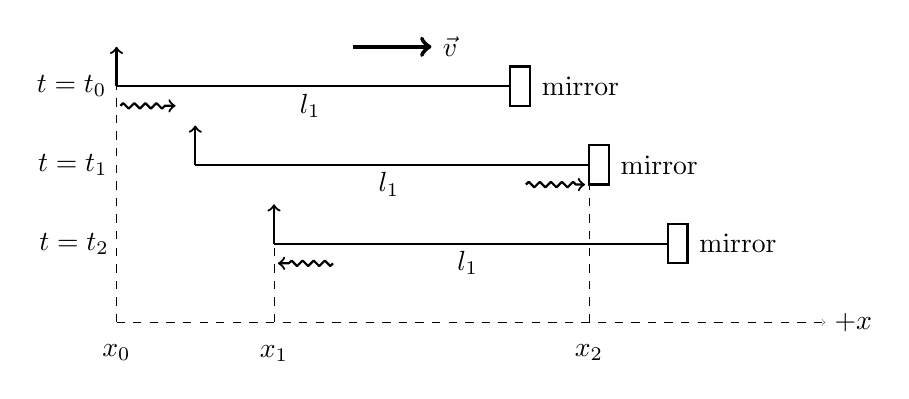
\begin{tikzpicture}[thick]
	    %speed vector + length
	    \draw [->, ultra thick] (3,0.5,0) -- (4,0.5,0) node[right] {\textbf{$\vec{v}$}};
	    %horizontal arrow
            \draw (5,0,0) -- (0,0,0) node[left] {$t=t_{0}$} node[right, xshift=150] {mirror} node[above, yshift=-15, xshift=70]{$l_{1}$};
            %vertical arrow
            \draw [->](0,0,0) -- (0,0.5,0);
            %mirror
            \draw (5,-0.25) rectangle (5.25,0.25);
            %squiggly arrow
            \draw [->, line join=round, decorate, decoration={zigzag, segment length=4, amplitude=1,post=lineto, post length=2pt}]  (0.05,-0.25,0) -- (0.75,-0.25,0);
            
            \draw (6,-1,0) -- (1,-1,0) node[left, xshift=-28] {$t=t_{1}$} node[right, xshift=150] {mirror} node[above, yshift=-15, xshift=70]{$l_{1}$};
            \draw [->](1,-1.0,0) -- (1,-0.5,0);
            \draw (6,-1.25) rectangle (6.25,-0.75);
            \draw [->, line join=round, decorate, decoration={zigzag, segment length=4, amplitude=1,post=lineto, post length=2pt}]  (5.20,-1.25,0) -- (5.95,-1.25,0);
            
            \draw (7,-2,0) -- (2,-2,0) node[left, xshift=-56] {$t=t_{2}$} node[right, xshift=150] {mirror} node[above, yshift=-15, xshift=70]{$l_{1}$};
            \draw [->](2,-2,0) -- (2,-1.5,0);
            \draw (7,-2.25) rectangle (7.25,-1.75);
            \draw [->, line join=round, decorate, decoration={zigzag, segment length=4, amplitude=1,post=lineto, post length=2pt}]  (2.75,-2.25,0) -- (2.05,-2.25,0);
            
            %x-axis
            \draw [->, dashed, ultra thin] (0,-3,0) -- (9,-3,0) node[right] {$+x$};
            %y-axes
            \draw[dashed, ultra thin] (0,-3,0) -- (0,0.0,.0) node[below, yshift = -90] {$x_{0}$};
            %\draw[dashed, ultra thin] (1,-3,0) -- (1,-1,0) node[below, yshift = -61.5, xshift = 29] {$x_{1}$};
            \draw[dashed, ultra thin] (2,-3,0) -- (2,-2,0) node[below, yshift = -33.5, xshift = 0] {$x_{1}$};
            \draw[dashed, ultra thin] (6,-3,0) -- (6,-1,0) node[below, yshift = -61.5, xshift = 0] {$x_{2}$};
    \end{tikzpicture}
    \caption{Horizontal arm, length $l_{1}$, moving with speed $v$ relative to the ``ether''}
    \label{fig: the horizontal}
  \end{figure}
  
  \noindent Our goal is to work out $\Delta t_{h}$, the time it takes for light to travel from $x_{0}$ to $x_{2}$, and $x_{2}$ back to $x_{1}$. Now, we can let the speed of light be $c$. We should also let $t_{a}=t_{1}-t_{0}$ and $t_{b}=t_{2}-t_{1}$. 
  
  \noindent First, we can easily obtain the time it takes for light to travel each path:
  
  \begin{equation} \label{eq:2.2}
  \begin{cases} 
  ct_{a}=l_{1}+vt_{a} \\
  ct_{b}=l_{1}-vt_{b} 
  \end{cases}
  \end{equation}
  
  \noindent Following some algebraic rearrangements, we get $t_{a}$ and $t_{b}$.
  \begin{equation} \label{eq:2.3}
  \begin{cases} 
  t_{a}=\frac{l_{1}}{c-v} \\
  t_{b}=\frac{l_{1}}{c+v} 
  \end{cases}
  \end{equation}
  
  \noindent Since the total time, $\Delta t_{h}$, is the sum of $t_{a}$ and $t_{b}$:
  \begin{equation} \label{eq:2.4} 
  \Delta t_{h}=t_{a}+t_{b}=\frac{l_{1}}{c-v}+\frac{l_{1}}{c+v}=\frac{2l_{1}c}{c^2-v^2}=\frac{2l_{1}}{c}.\frac{1}{1-\frac{v^2}{c^2}}
  \end{equation}
 
 \subsubsection{The ``vertical''}
   \begin{figure}[!h] %place figure here
 	\centering
 	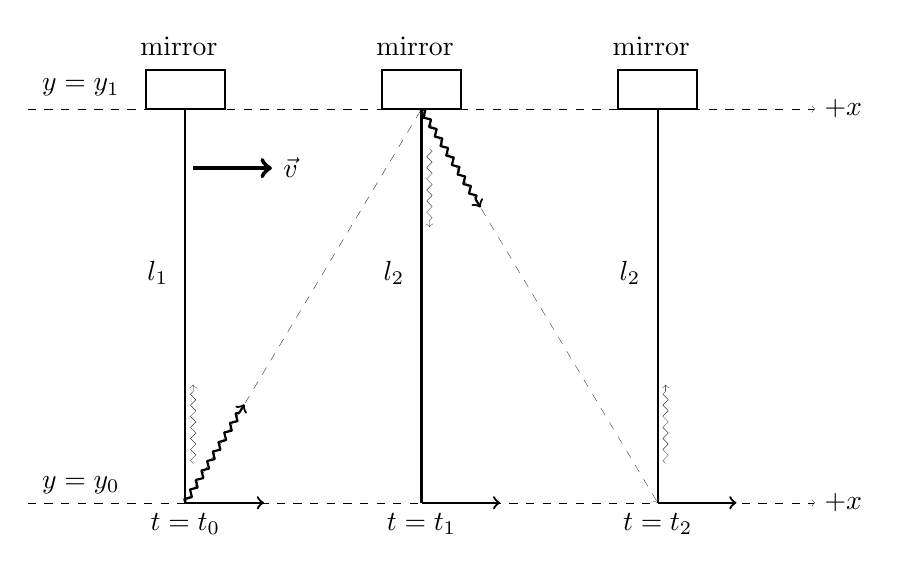
\begin{tikzpicture}[thick]
 	%speed vector + length
 	\draw [->, ultra thick] (0.1,4.25,0) -- (1.1,4.25,0) node[right] {\textbf{$\vec{v}$}};
 	
 	%horizontal arrow
 	\draw [->] (0,0,0) -- (1,0,0); 
 	%vertical arrow
 	\draw (0,5,0) -- (0,0,0) node[below] {$t=t_{0}$} node[right, yshift=165, xshift=-20] {mirror} node[above, yshift=75, xshift=-10]{$l_{1}$} node[left, xshift=-20, yshift=6.5]{$y=y_{0}$} node[left, xshift=-20, yshift=150]{$y=y_{1}$};
 	%mirror
 	\draw (-0.5,5) rectangle (0.5,5.5);
 	%squiggly arrow
 	\draw [->, line join=round, ultra thin, decorate, decoration={zigzag, segment length=4, amplitude=1,post=lineto, post length=2pt}]  (0.1,0.5,0) -- (0.1,1.5,0);
 	
 	%horizontal arrow
 	\draw [->] (3,0,0) -- (4,0,0); 
 	%vertical arrow
 	\draw (3,5,0) -- (3,0,0) node[below] {$t=t_{1}$} node[right, yshift=165, xshift=-20] {mirror} node[above, yshift=75, xshift=-10]{$l_{2}$};
 	%mirror
 	\draw (2.5,5) rectangle (3.5,5.5);
 	%squiggly arrow
 	\draw [->, line join=round, ultra thin, decorate, decoration={zigzag, segment length=4, amplitude=1,post=lineto, post length=2pt}] (3.1,4.5,0) -- (3.1,3.5,0);
 	
 	%horizontal arrow
 	\draw [->] (6,0,0) -- (7,0,0); 
 	%vertical arrow
 	\draw (6,5,0) -- (6,0,0) node[below] {$t=t_{2}$} node[right, yshift=165, xshift=-20] {mirror} node[above, yshift=75, xshift=-10]{$l_{2}$};
 	%mirror
 	\draw (5.5,5) rectangle (6.5,5.5);
 	%squiggly arrow
 	\draw [->, line join=round, ultra thin, decorate, decoration={zigzag, segment length=4, amplitude=1,post=lineto, post length=2pt}]  (6.1,0.5,0) -- (6.1,1.5,0);
 	
 	%"up"
 	\draw [->, dashed, ultra thin] (0,0,0) -- (3,5,0) node[right] {};
 	%"down"
 	\draw [->, dashed, ultra thin] (3,5,0) -- (6,0,0) node[right] {};
 	
 	%"up arrow"
 	\draw [->, line join=round, decorate, decoration={zigzag, segment length=4, amplitude=1,post=lineto, post length=2pt}]  (0,0,0) -- (0.75,1.25,0);
 	%"down arrow"
 	\draw [->, line join=round, decorate, decoration={zigzag, segment length=4, amplitude=1,post=lineto, post length=2pt}]  (3,5,0) -- (3.75,3.75,0);
 	
 	%x-axess
 	\draw [->, dashed, ultra thin] (-2,0,0) -- (8,0,0) node[right] {$+x$};
 	\draw [->, dashed, ultra thin] (-2,5,0) -- (8,5,0) node[right] {$+x$};
 	
 
 	\end{tikzpicture}
 	\caption{Vertical arm, length $l_{2}$, moving with speed $v$ relative to the ``ether''}
 	\label{fig: the vertical}
 \end{figure}
 
 \noindent Our goal, similar that in the previous section, is to work out $\Delta t_{v}$, the time it takes for light to travel from $y_{0}$ to $y_{1}$, and $y_{1}$ back to $y_{0}$. Let $t_{c}=t_{1}-t_{0}$ and $t_{d}=t_{2}-t_{1}$. 
 
 \noindent Again, we obtain the time it takes for light to travel each path. However, note that the light paths in this case are different from those in the "horizontal" scenario. From the ground frame, light travels diagonal paths, as illustrated in Figure \ref{fig: the vertical} as dashed lines, rather than along the vertical arm of the interferometer. Hence, we use the Pythagorean theorem to find the path length.
 \begin{equation} \label{eq:2.5}
 \begin{cases} 
 ct_{c}=\sqrt{{l_{2}}^{2} - {(vt_{c})}^{2}} \\
 ct_{d}=\sqrt{{l_{2}}^{2} - {(vt_{d})}^{2}} 
 \end{cases}
 \end{equation}
 
 \noindent Following some algebraic rearrangements, we obtain $t_{c}$ and $t_{d}$. Not surprisingly, these two quantities are equal.
 \begin{equation} \label{eq:2.6} 
 t_{c}=t_{d}=\frac{l_{2}}{c}.\frac{1}{\sqrt{1-\frac{v^2}{c^2}}}  
 \end{equation}
 
 \noindent Again, we obtain $\Delta t_{v}$ by summing $t_{c}$ and $t_{d}$.
 \begin{equation} \label{eq:2.7}
 \Delta t_{v}=t_{c}+t_{d}=\frac{2l_{2}}{c}.\frac{1}{\sqrt{1-\frac{v^2}{c^2}}}
 \end{equation}
 
 \subsubsection{Michelson's first brilliant observation}
 Suppose that the speed $v$ at which the interferometer travels relative to the "ether" is approximately the speed at which Earth orbits the Sun, the speed of light $c$ is so great compared to $v$ that $\Delta t_{h} \approx \Delta t_{v}$, and thus any difference between $\Delta t_{h}$ and  $\Delta t_{v}$ would be humanly undetectable. 
 
 \noindent However, Michelson's use of interferometry allows for detections of slightest time differences between the vertical and horizontal arms. Interferometry, as its name suggests, works based on the ability of light to interfere. Differences between $\Delta t_{h}$ and  $\Delta t_{v}$, if they existed, would result in constructive and destructive interference, creating detectable "fringes." Hence, if "fringes" were observed, Michelson would be able to confirm that existence of the ``luminiferous ether.''  
 
 \subsubsection{Michelson's second brilliant observation}
 Michelson's second brilliant idea is to rotate the interferometer, alternating the roles of the vertical and horizontal arms - vertical becoming horizontal, horizontal becoming vertical. 
 
 \noindent The purpose of alternating the roles of the vertical and horizontal arms of the interferometer is to create visible "fringe shifts." Mathematically speaking, rotating the apparatus allows for the removal of the speed of light $c$ from part of the calculations and for the fractional time differences to be dependent only on the sum of the arm lengths rather than individual arm lengths, thus simplifying the machining and detection process. 
 
 \noindent While there are infinitely many angles the apparatus can be rotated relative to its original position, we can fully show the effect of rotating the interferometer by considering special cases, when $\theta=\ang{0}$ and $\theta=\ang{90}$.
 
 \noindent First, we consider $\theta=\ang{0}$. We are interested in the difference between the time light takes in the vertical ($\Delta t_{v_{0}}$) versus horizontal arms ($\Delta t_{h_{0}}$). We shall call this quantity $\Delta t_{\ang{0}}$.
 \begin{equation} \label{eq:2.8}
 \Delta t_{\ang{0}}=\Delta t_{v_{0}}-\Delta t_{h_{0}}=\frac{2l_{2}}{c}.\frac{1}{\sqrt{1-\frac{v^2}{c^2}}}-\frac{2l_{1}}{c}.\frac{1}{1-\frac{v^2}{c^2}}
 \end{equation} 
 Now, let's consider $\Delta t_{\ang{90}}$:
 \begin{equation} \label{eq:2.9}
 \Delta t_{\ang{90}}=\Delta t_{v_{90}}-\Delta t_{h_{90}}=\frac{2l_{2}}{c}.\frac{1}{1-\frac{v^2}{c^2}}-\frac{2l_{1}}{c}.\frac{1}{\sqrt{1-\frac{v^2}{c^2}}}
 \end{equation}
 \noindent What we are interested now the difference between the time differences at $\Delta t_{\ang{0}}$ and $\Delta t_{\ang{90}}$. Let this quantity be $\Delta t$.
 \begin{equation}\label{eq:2.10}
 \Delta t=\Delta t_{\ang{90}}-\Delta t_{\ang{0}}=\frac{2}{c}(l_{1}+l_{2})\left(\frac{1}{1-\frac{v^2}{c^2}} - \frac{1}{\sqrt{1-\frac{v^2}{c^2}}}\right)
 \end{equation}
 \noindent By now, we must have found the term $\frac{v^2}{c^2}$ quite ubiquitous. So, we can (in fact we really should) assign to it a more elegant symbol $\beta$. \eqref{eq:2.10} now becomes:
 \begin{equation}\label{eq:2.11}
 \Delta t=\Delta t_{\ang{90}}-\Delta t_{\ang{0}}=\frac{2}{c}(l_{1}+l_{2})\left(\frac{1}{1-{\beta}^{2}} - \frac{1}{\sqrt{1-{\beta}^{2}}}\right)
 \end{equation}
 Since $v\ll c$, or in other words $\beta \ll 1$, we can simplify \eqref{eq:2.11} by approximating the terms containing $\beta$. Specifically, we are using the following approximation,
 \begin{equation}\label{eq:2.12}
 (1+x)^{p}\approx1+px
 \end{equation}
 for $x \ll 1$, to obtain a simpler version of \eqref{eq:2.11}:
 \begin{equation}\label{eq:2.13}
 \begin{split}
 \Delta t&=\frac{2}{c}(l_{1}+l_{2})\left(\frac{1}{1-{\beta}^{2}} - \frac{1}{\sqrt{1-{\beta}^{2}}}\right) \\
 &\approx\frac{2}{c}(l_{1}+l_{2})\left[(1+{\beta}^{2}) - \left(1+\frac{1}{2}{\beta}^{2}\right)\right] \\
 &= \left(\frac{l_{1}+l_{2}}{c}\right){\beta}^{2}
 \end{split}
 \end{equation}
 \noindent Now, in order to achieve maximum "fringe shifts," we (or Michelson more exactly) would want to have the time difference $\Delta t$ to be half the "period of light" - meaning that light on one path travels a half wavelength more than light on the other path. Hence, we can let:
 \begin{equation}\label{eq:2.14}
 \begin{split}
 \frac{\Delta t}{T}&=\left(\frac{l_{1}+l_{2}}{c}\right){\beta}^{2}\left(\frac{c}{\lambda}\right) \\
 &=\left(\frac{l_{1}+l_{2}}{\lambda}\right){\beta}^{2}=0.5
 \end{split}
 \end{equation}
 where $\lambda = \SI{590}{\nano\meter}$ is the wavelength of the sodium source which Michelson used in his experiment and $T=\frac{1}{\nu}=\frac{\lambda}{c}$ is the "period" of light.
 
 \noindent Earlier, we made an assumption that $v$ is the speed of the Earth around the Sun. Hence, $\beta\approx 10^{-4}$. So, to take $\frac{\Delta t}{T} \approx 0.5$, the sum of the arm lengths should be around $20-30 \SI{}{\meter}$, which was totally achievable in a laboratory setting. In fact, Michelson chose to make the arm lengths $\SI{11}{\meter}$ each, which, if the "ether" hypothesis were true, should give $\frac{\Delta t}{T} \approx 0.4$. 
 
 \noindent As it turned out, however, Michelson did not detect any changes in the interference patterns. In fact, he found that $\frac{\Delta t}{T} <  0.005$.
 
 \subsection{A different experiment: Bradley's Stellar Aberration (1725)}
 A different experiment, on the other hand, gave results in agreement with the "ether drift" theory. 
 
 \noindent Astronomers in the 18\textsuperscript{th} century realized they had to tilt their telescopes by some angle $\alpha$ away from the direction in which light was coming towards their location $\theta$, in order to be able to see the stars. We immediately obtain the relationship:
 \begin{equation} \label{eq:2.15}
 \alpha = \theta - {\theta}^{\prime}
 \end{equation}
 
  \begin{figure}[htb] %place figure here
 	\centering
 	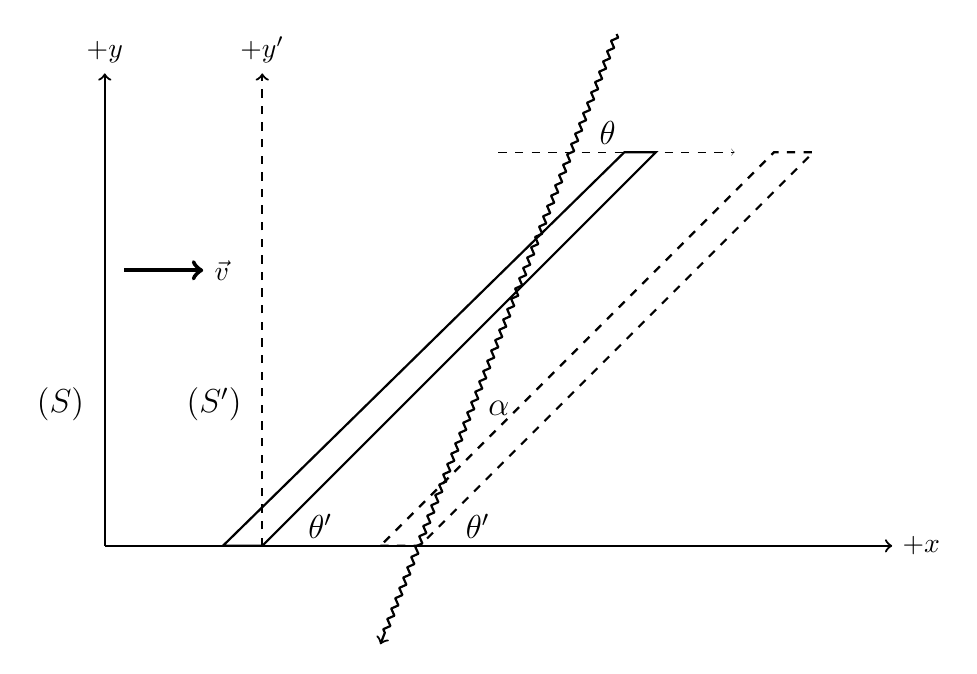
\begin{tikzpicture}[->, thick]
 	\draw (0,0,0) -- (0,6,0) node[above] {$+y$}; %+Y
 	\draw [dashed](2,0,0) -- (2,6,0) node[above] {$+y'$}; %+y'
 	\draw (0,0,0) -- (10,0,0) node[right] {$+x$}; %+x
 	\draw [dashed, ultra thin] (5,5,0) -- (8,5,0); %+x---
 	%\draw (0,0,0) -- (0,0,3.5) node[left] {$+z$}; %z
 	%\draw (5,0,0) -- (5,0,3.5) node[left] {$+z'$}; %z'
 	
 	%velocity vector
 	\draw [->, ultra thick] (0.25,3.5,0) -- (1.25,3.5,0) node[right] {\textbf{$\vec{v}$}};
 	
 	%frame marker
 	\node[label={left: \large ${(S)}$}] at (0,1.80,0){};
 	\node[label={left: \large ${(S')}$}] at (2,1.80,0){};
 	
 	%angle marker
 	\node[label={left: \large${\theta}^{\prime}$}] at (3.15, 0.25,0) {};
 	\node[label={left: \large${\theta}^{\prime}$}] at (5.15, 0.25,0) {};
 	\node[label={left: \large$\alpha$}] at (5.40, 1.75,0) {};
 	\node[label={left: \large$\theta$}] at (6.75, 5.25,0) {};
 	
 	%telescopes
 	\draw (1.5,0) -- (2,0) -- (7,5) -- (6.6,5) -- cycle;
 	\draw [dashed] (3.5,0) -- (4,0) -- (9,5) -- (8.5,5) -- cycle;
 	
 	%light, squiggly arrow
 	\draw [->, line join=round, decorate, decoration={zigzag, segment length=4, amplitude=1,post=lineto, post length=4pt}] (6.5,6.5) -- (3.5,-1.25);
 	
 	\end{tikzpicture}
 	\caption{Bradley's stellar aberration set-up (1725) (exaggerated)}
 	\label{fig: stellar aberration}
 \end{figure}
 \noindent While not absolutely necessary, we should take a peek at how the angle ${\theta}^{\prime}$ can be calculated. We will not go into detail how the following expression is obtained. However, its derivation is rather simple solution to a geometry problem. 
 \begin{equation} \label{eq:2.16}
 \frac{{u_{x}}^{\prime}}{u}=\cos({\theta}^{\prime})=\frac{u\cos(\theta)-v}{\sqrt{u^2+v^2-2uv\cos(\theta)}}
 \end{equation}  
 \noindent where $u$ is the speed of light $c$, and ${u_{x}}^{\prime}$ is the speed of light in the $x$-direction, in the moving frame. Now, we shall consider the case in which star light is coming straight down, making a $\ang{90}$ angle with the horizontal:
 \begin{equation} \label{eq:2.17}
 \cos({\theta}^{\prime})=\left(\frac{-v}{c}\right)\frac{1}{\sqrt{1+\frac{v^2}{c^2}}}\approx -\frac{v}{c}
 \end{equation}
 which makes a lot of geometric sense. (This is similar to the raindrop problem).
 
 \newpage
 
 \section{Einstein's Postulates of Relativity}
 Can we reconcile the Michelson-Morley experiment and Bradley's Stellar Aberration? Are the laws of Electricity and Magnetism independent of any inertial frame?
 \subsection{Einstein's realization about electricity and magnetism}
 \indent Einstein's theory of special relativity came about as a result of his studying Maxwell's equations of electricity and magnetism. In fact, in his first paper on special relativity - \textit{On the Electrodynamics of Moving Bodies}, published in his golden years (\textit{Annus Mirabilis}), Einstein wrote:\smallskip\\
 \indent ``It is known that Maxwell\textquoteright s electrodynamics\textemdash as usually understood at the present time\textemdash when applied to moving bodies, leads to asymmetries which do not appear to be inherent in the phenomena. Take, for example, the reciprocal electrodynamic action of a magnet and a conductor. The observable phenomenon here depends only on the relative motion of the conductor and the magnet, whereas the customary view draws a sharp distinction between the two cases in which either the one or the other of these bodies is in motion. For if the magnet is in motion and the conductor at rest, there arises in the neighbourhood of the magnet an electric field with a certain definite energy, producing a current at the places where parts of the conductor are situated. But if the magnet is stationary and the conductor in motion, no electric field arises in the neighbourhood of the magnet. In the conductor, however, we find an electromotive force, to which in itself there is no corresponding energy, but which gives rise\textemdash assuming equality of relative motion in the two cases discussed\textemdash to electric currents of the same path and intensity as those produced by the electric forces in the former case.''
 
 \noindent Essentially, what Einstein realizes from studying Maxwell's equations is that Electricity and Magnetism are two sides of the same coin.
 
 \subsection{Postulates of Special Relativity}
 %Here it comes... The real deal.
 \subsubsection{Einsteins postulates}
 (a) All laws of physics are the \textbf{same} in all inertial reference frames. In other words, all laws of physics must retain their mathematical forms regardless of any reference frames in which they are considered.\smallskip\\
 (b) The speed of light is the \textbf{same} in all inertial reference frames. This postulate is also called the \textit{The Principle of the Constancy of the Speed of Light}. This means the speed of light is always measured to be $c$, independent of reference frames. For example, both you (standing on Earth) and the I.S.S. (which is orbiting Earth at dazzling speeds) agree that $c=\SI{299 792 458}{\meter\per\second}$. 
 
 \newpage 
 
 \section{Fundamental consequences of the postulates} 
 This is the prelude to the ``Lorentz-Einstein Transformation,'' a very useful mathematical tool for solving special relativity problems. However, before we can into more rigorous and ``mathy'' meat of special relativity, we will first discuss the consequences of Einstein's postulates\textemdash in order to gain a better understanding of the rules of special relativity and hopefully develop some intuition and prepare our minds for the less intuitive stuff ahead.  
 \subsection{Relativity of Simultaneity}
 In this section, we will attempt to answer whether simultaneous events in some frame $(S)$ remain simultaneous in some other frame $(S')$ that is moving with speed $v$ relative to $(S)$. In order to do so, let's meet Alice and Bob, our lab assistants:
 %add Alice and Bob here
 \begin{figure}[htb]
 \centering
 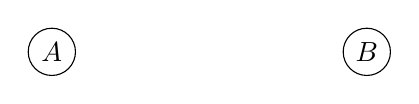
\begin{tikzpicture}
  \draw (0,0) circle [radius=0.3] node {$A$};
  \draw (4,0) circle [radius=0.3] node {$B$};
 \end{tikzpicture}
 \end{figure}

 \noindent It's okay if you are socially awkward. You'll see them enough times that greetings will eventually become unnecessary. Anyway, consider the following situation: Alice is in a train moving at speed $v$ relative to the ground. Bob stands on the ground. A light source in the middle of Alice's car fires two pulses in opposite directions, parallel to the train's direction of motion.\smallskip\\
 \noindent For Alice, the two pulses arrive at the ends of the train simultaneously, illustrated below:
 \begin{figure}[htb] 
 	\centering
 	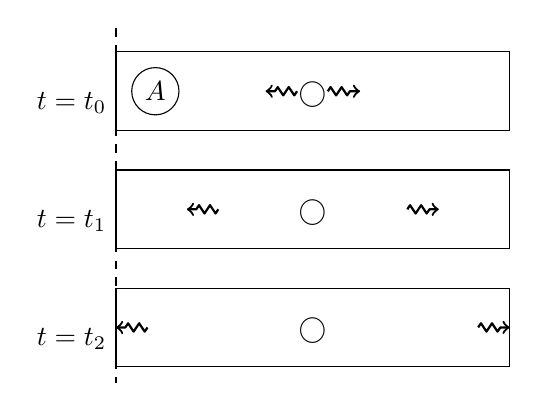
\begin{tikzpicture}
 	
 	\draw (0,0)--(5,0)--(5,1)--(0,1)--cycle node[left, yshift=10]{$t=t_{0}$} node[above, xshift=71, yshift=5] {$ \bigcirc $};
 	\draw [->, thick, line join=round, decorate, decoration={zigzag, segment length=4, amplitude=1.5,post=lineto, post length=2pt}] (2.3,.5) -- (1.9,.5);
 	\draw [->, thick, line join=round, decorate, decoration={zigzag, segment length=4, amplitude=1.5,post=lineto, post length=2pt}] (2.69,.5) -- (3.1,.5);
 	
 	\draw (0,-1.5)--(5,-1.5)--(5,-0.5)--(0,-0.5)--cycle node[left, yshift=10]{$t=t_{1}$} node[above, xshift=71, yshift=5] {$ \bigcirc $};
 	\draw [->, thick, line join=round, decorate, decoration={zigzag, segment length=4, amplitude=1.5,post=lineto, post length=2pt}] (1.3,-1) -- (0.9,-1);
 	\draw [->, thick, line join=round, decorate, decoration={zigzag, segment length=4, amplitude=1.5,post=lineto, post length=2pt}] (3.7,-1) -- (4.1,-1);
 	
 	\draw (0,-3)--(5,-3)--(5,-2)--(0,-2)--cycle node[left, yshift=10] {$t=t_{2}$} node[above, xshift=71, yshift=5] {$\bigcirc$};
 	\draw [->, thick, line join=round, decorate, decoration={zigzag, segment length=4, amplitude=1.5,post=lineto, post length=2pt}] (0.4,-2.5) -- (0,-2.5);
 	\draw [->, thick, line join=round, decorate, decoration={zigzag, segment length=4, amplitude=1.5,post=lineto, post length=2pt}] (4.6,-2.5) -- (5,-2.5);
 	
 	%Alice and +y, t=0 line
 	\draw [dashed](0,1.3) -- (0,-3.2);
 	\draw (0.5,0.5) circle [radius=0.3] node {$A$};
 	
 	\end{tikzpicture}
 	\caption{Alice's train in Alice's frame, over time}
 	\label{fig: alice's frame 1}
 \end{figure}

 \noindent For Bob, however, things are little different. According to Einstein's second postulate of relativity, the speed of light is constant. Therefore, we should expect that Bob, in the ground frame, sees the left pulse arrive at the end of Alice's train \textbf{before} the right pulse arrive at the other end. As we visualize the problem, it becomes fairly obvious that simultaneous events in Alice's frame are not simultaneous in Bob's frame.
 \begin{figure}[htb] 
 	\centering
 	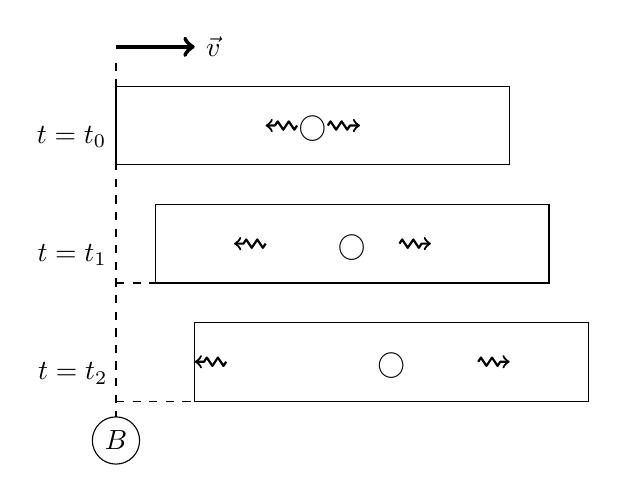
\begin{tikzpicture}
 	
 	\draw (0,0)--(5,0)--(5,1)--(0,1)--cycle node[left, yshift=10]{$t=t_{0}$} node[above, xshift=71, yshift=5] {$ \bigcirc $};
 	\draw [->, thick, line join=round, decorate, decoration={zigzag, segment length=4, amplitude=1.5,post=lineto, post length=2pt}] (2.3,.5) -- (1.9,.5);
 	\draw [->, thick, line join=round, decorate, decoration={zigzag, segment length=4, amplitude=1.5,post=lineto, post length=2pt}] (2.69,.5) -- (3.1,.5);
 	
 	\draw (0.5,-1.5)--(5.5,-1.5)--(5.5,-0.5)--(0.5,-0.5)--cycle node[left, yshift=10, xshift=-14]{$t=t_{1}$} node[above, xshift=71, yshift=5] {$ \bigcirc $};
 	\draw [->, thick, line join=round, decorate, decoration={zigzag, segment length=4, amplitude=1.5,post=lineto, post length=2pt}] (1.9,-1) -- (1.5,-1);
 	\draw [->, thick, line join=round, decorate, decoration={zigzag, segment length=4, amplitude=1.5,post=lineto, post length=2pt}] (3.6,-1) -- (4,-1);
 	
 	\draw (1,-3)--(6,-3)--(6,-2)--(1,-2)--cycle node[left, yshift=10, xshift=-28] {$t=t_{2}$} node[above, xshift=71, yshift=5] {$\bigcirc$};
 	\draw [->, thick, line join=round, decorate, decoration={zigzag, segment length=4, amplitude=1.5,post=lineto, post length=2pt}] (1.4,-2.5) -- (1,-2.5);
 	\draw [->, thick, line join=round, decorate, decoration={zigzag, segment length=4, amplitude=1.5,post=lineto, post length=2pt}] (4.6,-2.5) -- (5,-2.5);
 	
 	%Bob and +y, t=0 line
 	\draw [dashed](0,1.3) -- (0,-3.2);
 	\draw [dashed](0,-1.5) -- (0.5,-1.5);
 	\draw [dashed](0,-3) -- (1,-3);
 	\draw (0,-3.5) circle [radius=0.3] node {$B$};
 	
 	%velocity vector
 	\draw [->, ultra thick] (0,1.5) -- (1,1.5) node[right] {\textbf{$\vec{v}$}};
 	
 	\end{tikzpicture}
 	\caption{Alice's train in Bob's frame, over time}
 	\label{fig: bob's frame 1}
 \end{figure} 
 
 \noindent This visualization certainly useful - because it approximates very well what happens in space at certain points in time. However, the sketching process can become too tedious when we deal with more complex relativity problems that involves more relatively moving objects. An alternative and more effective route to visualizing relativity problem, as we have touched on earlier, is drawing spacetime diagrams: one for Alice, one for Bob. For Alice's diagram, we can see that the pulses arrive at the rear and front of the train at the same time.
 \begin{figure}[!htb] %place figure here
 	\centering
 	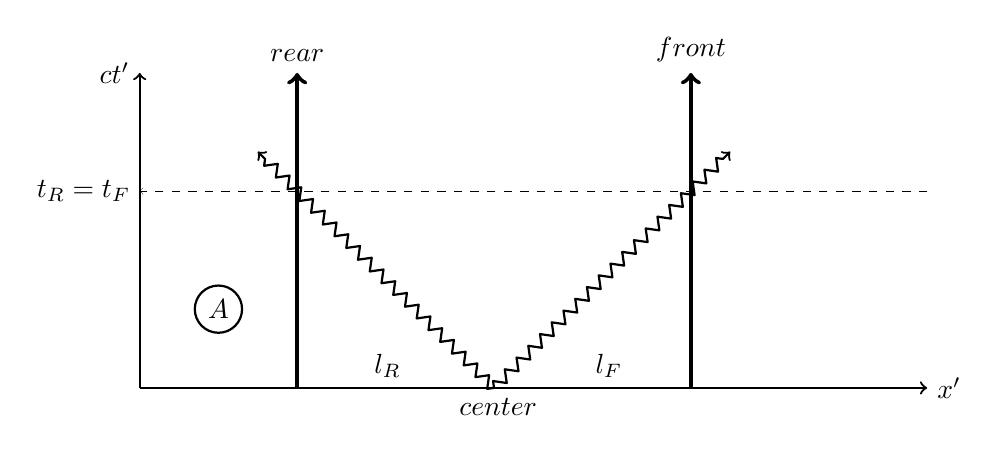
\begin{tikzpicture}[->, thick]
 	\draw (0,0,0) -- (0,4,0) node[left] {$ct'$}; %+Y
 	\draw [ultra thick](2,0,0) -- (2,4,0) node[above] {$rear$}; %+y'
 	\draw [ultra thick](7,0,0) -- (7,4,0) node[above] {$front$}; %+y'
 	
 	%horizontal axis
 	\draw (0,0,0) -- (10,0,0) node[right] {$x'$} node[above, xshift=-195] {$l_{R}$} node[above, xshift=-115]{$l_{F}$} node[below, xshift=-155]{$center$}; %+x'
 	
 	
 	\draw [dashed, ultra thin] (10,2.5) -- (0,2.5,0) node[left]{$t_{R}=t_{F}$}; %+x---
 	
 	% light arrows
 	\draw [->, line join=round, decorate, decoration={zigzag, segment length=6, amplitude=2,post=lineto, post length=2pt}] (4.5,0) -- (1.5,3);
 	\draw [->, line join=round, decorate, decoration={zigzag, segment length=6, amplitude=2,post=lineto, post length=2pt}] (4.5,0) -- (7.5,3);
 	
 	%Alice's name:
 	\draw (1,1) circle [radius=0.3] node {$A$};
 	
 	\end{tikzpicture}
 	\caption{Alice's spacetime diagram}
 	\label{fig: alice's spacetime 1}
 \end{figure}

 \noindent As we have shown earlier, this (simultaneity) is not the case in Bob's frame. In fact, the left pulse hits the \textbf{rear} of the Alice's train \textbf{before} the right pulse hits the \textbf{front} of the train. 
 \begin{figure}[!htb] %place figure here
 	\centering
 	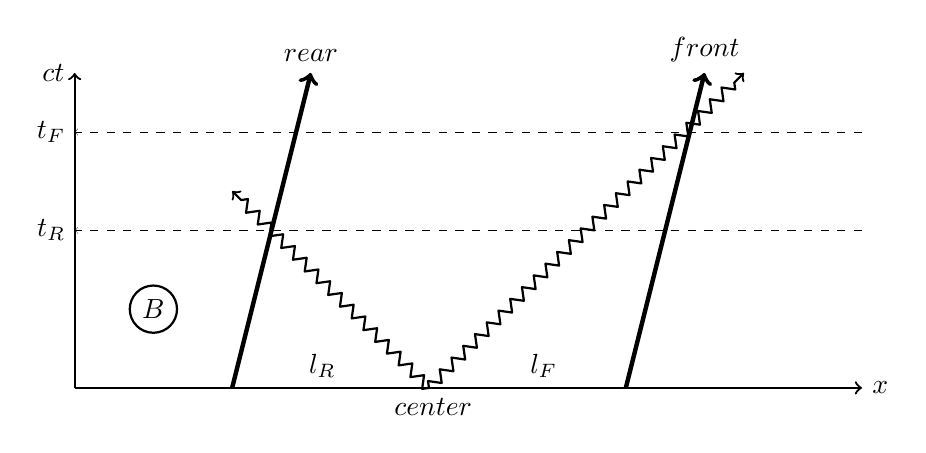
\begin{tikzpicture}[->, thick]
 	\draw (0,0,0) -- (0,4,0) node[left] {$ct$}; %+Y
 	\draw [ultra thick](2,0,0) -- (3,4,0) node[above] {$rear$}; %+y'
 	\draw [ultra thick](7,0,0) -- (8,4,0) node[above] {$front$}; %+y'
 	
 	\draw (0,0,0) -- (10,0,0) node[right] {$x$} node[above, xshift=-195] {$l_{R}$} node[above, xshift=-115]{$l_{F}$} node[below, xshift=-155]{$center$}; %+x
 	
 	\draw [dashed, ultra thin] (10,2) -- (0,2) node[left]{$t_{R}$}; %+x---
 	\draw [dashed, ultra thin] (10,3.25) -- (0,3.25) node[left]{$t_{F}$}; %+x---
 	
 	% light arrows
 	\draw [->, line join=round, decorate, decoration={zigzag, segment length=6, amplitude=2,post=lineto, post length=2pt}] (4.5,0) -- (2,2.5);
 	\draw [->, line join=round, decorate, decoration={zigzag, segment length=6, amplitude=2,post=lineto, post length=2pt}] (4.5,0) -- (8.5,4);
 	
 	%Bob's name:
 	\draw (1,1) circle [radius=0.3] node {$B$};
 	
 	\end{tikzpicture}
 	\caption{Bob's spacetime diagram}
 	\label{fig: bob's spacetime 1}
 \end{figure}

 \noindent Now that we know simultaneity is not independent of reference frames, we shall attempt to find the difference between the pulses' arrival times. We shall stick with our previous setup, with a little change. For later convenience, we will change the location of the light source in the train so that the pulses arrive at the front and rear of Alice's train \textbf{simultaneously} in Bob's frame. Hence, we should re-draw Alice's and Bob's spacetime diagrams.
 \begin{figure}[!htb] %place figure here
 	\centering
 	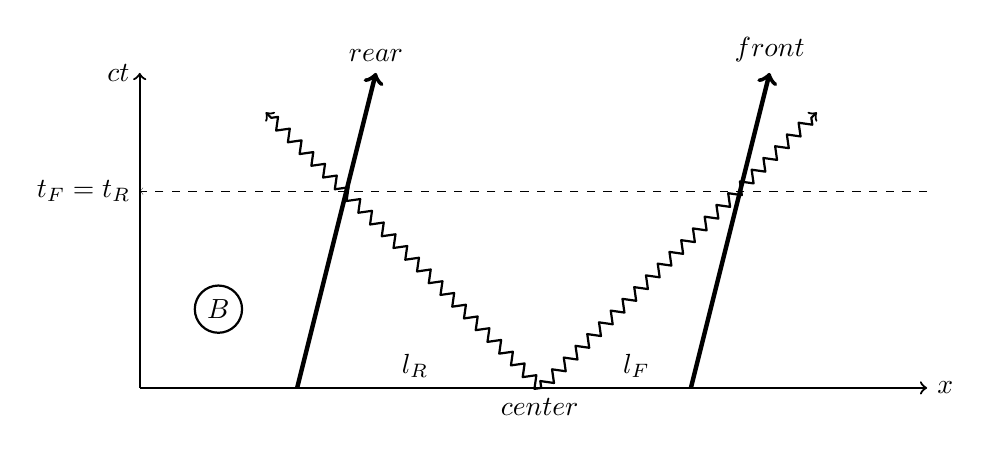
\begin{tikzpicture}[->, thick]
 	\draw (0,0,0) -- (0,4,0) node[left] {$ct$}; %+Y
 	\draw [ultra thick](2,0,0) -- (3,4,0) node[above] {$rear$}; %+y'
 	\draw [ultra thick](7,0,0) -- (8,4,0) node[above] {$front$}; %+y'
 	\draw (0,0,0) -- (10,0,0) node[right] {$x$} node[above, xshift=-185] {$l_{R}$} node[above, xshift=-105]{$l_{F}$} node[below, xshift=-140]{$center$}; %+x

	%arrival time
 	\draw [dashed, ultra thin] (10,2.5) -- (0,2.5) node[left]{$t_{F}=t_{R}$}; %+x---

 	% light arrows
 	\draw [->, line join=round, decorate, decoration={zigzag, segment length=6, amplitude=2,post=lineto, post length=2pt}] (5.1,0) -- (1.6,3.5);
 	\draw [->, line join=round, decorate, decoration={zigzag, segment length=6, amplitude=2,post=lineto, post length=2pt}] (5.1,0) -- (8.6,3.5);
 	
 	%Bob's name:
 	\draw (1,1) circle [radius=0.3] node {$B$};
 	
 	\end{tikzpicture}
 	\caption{Bob's new spacetime diagram}
 	\label{fig: bob's spacetime 2}
 \end{figure}

 \noindent Since the light pulses arrive the ends of Alice's train simultaneously in Bob's frame, we can write $l_{r}$ and $l_{f}$ in terms of the length of the train, in Bob's frame, $L_{B}$. We have the following system of equations to start: 
 \begin{equation}\label{eq:4.1}
 \begin{cases}
 l_{R} + l_{F} = L_{B} \\
 t_{R} = t_{F}\\
 ct_{R} = l_{R} - vt_{R}\\
 ct_{L} = l_{L} + vt_{L}
 \end{cases}
 \end{equation}
 
 \noindent With a little bit of algebraic rearrangements, we can figure out how $L_{B}$ should be divided so that the light pulses reach the ends of Alice's train simultaneously in Bob's frame:
 \begin{equation}\label{eq:4.2}
 \begin{cases}
 l_{F}=\frac{L_{B}}{2}\left(1-\frac{v}{c}\right)\\
 l_{R}=\frac{L_{B}}{2}\left(1+\frac{v}{c}\right)
 \end{cases}
 \end{equation}
 
 \noindent This is also how $L_{A}$ is divided in Alice's frame. 
 \begin{figure}[!htb] %place figure here
 	\centering
 	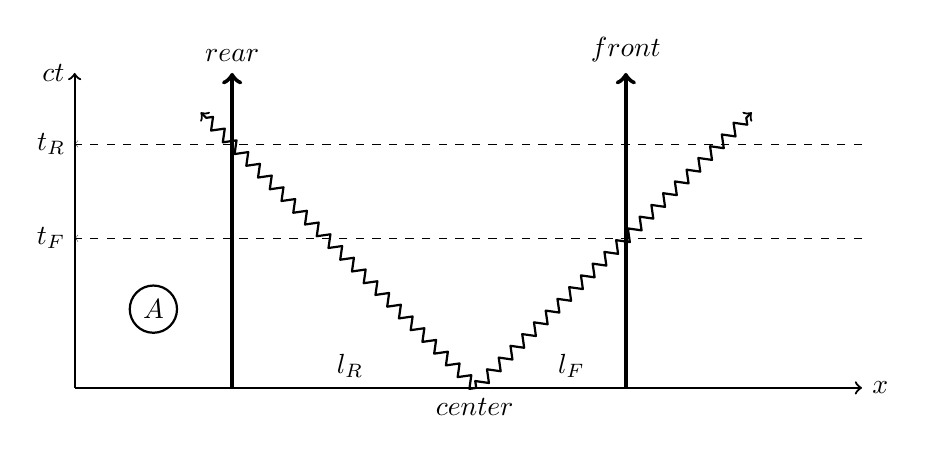
\begin{tikzpicture}[->, thick]
 	\draw (0,0,0) -- (0,4,0) node[left] {$ct$}; %+Y
 	\draw [ultra thick](2,0,0) -- (2,4,0) node[above] {$rear$}; %+y'
 	\draw [ultra thick](7,0,0) -- (7,4,0) node[above] {$front$}; %+y'
 	
 	\draw (0,0,0) -- (10,0,0) node[right] {$x$} node[above, xshift=-185] {$l_{R}$} node[above, xshift=-105]{$l_{F}$} node[below, xshift=-140]{$center$}; %+x
 	
 	%arrival times
 	\draw [dashed, ultra thin] (10,1.9) -- (0,1.9) node[left]{$t_{F}$}; %+x---
 	\draw [dashed, ultra thin] (10,3.1) -- (0,3.1) node[left]{$t_{R}$}; %+x--- %+x---
 	
 	% light arrows
 	\draw [->, line join=round, decorate, decoration={zigzag, segment length=6, amplitude=2,post=lineto, post length=2pt}] (5.1,0) -- (1.6,3.5);
 	\draw [->, line join=round, decorate, decoration={zigzag, segment length=6, amplitude=2,post=lineto, post length=2pt}] (5.1,0) -- (8.6,3.5);
 	
 	%Alice's name:
 	\draw (1,1) circle [radius=0.3] node {$A$};
 	
 	\end{tikzpicture}
 	\caption{Alice's new spacetime diagram}
 	\label{fig: alice's spacetime 2}
 \end{figure}

 \noindent We can express $l_{R}$ and $l_{F}$ in Alice's frame in terms of $L_{A}$, $v$, and $c$. 
 \begin{equation}\label{eq:4.3}
 \begin{cases}
 l_{F}=c{t_{F}}^{\prime}=\frac{L_{A}}{2}\left(1-\frac{v}{c}\right)\\
 l_{R}=c{t_{R}}^{\prime}=\frac{L_{A}}{2}\left(1+\frac{v}{c}\right)
 \end{cases}
 \end{equation}
 
 \noindent Now we can write down the expression for the time interval between the pulses' arrivals in Alice's frame:
 \begin{equation}\label{eq:4.4}
 \Delta t^{\prime}={t_{R}}^{\prime}-{t_{F}}^{\prime}=\frac{L_{A}v}{c^2}
 \end{equation}
 
 \noindent Keep in mind that all of the calculations we have been doing are in Bob's frame. More specifically, we based all of our derivations on events that are simultaneous in Bob's frame. What we found, according to \eqref{eq:4.4}, is that Bob sees not only the \textbf{loss of simultaneity} in Alice's frame, but also Alice's rear clock giving larger reading than Alice's front clock. This is another fundamental effect of Einstein's postulates: \textbf{rear clock ahead}, which we will visualize and simplify in the following section.
 \subsubsection{Simultaneity and clock readings}
 The diagram below sums up what happens to Alice's clock readings \textbf{in Bob's frame}. 
 
 \begin{figure}[!htb]
 	\centering
 	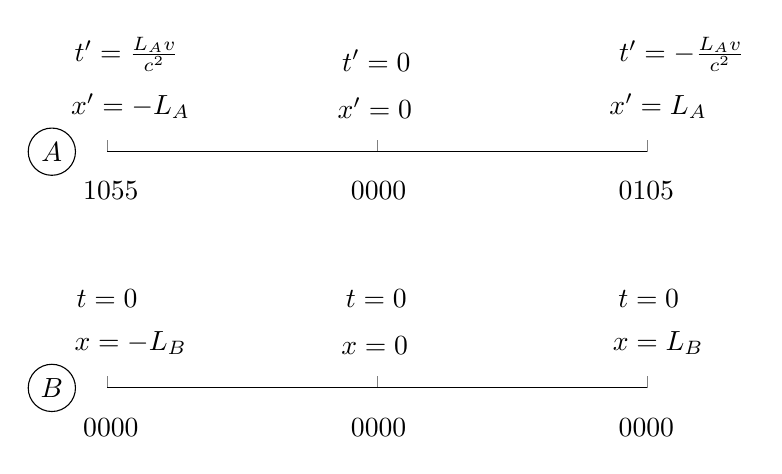
\begin{tikzpicture}
 	
 	%Alice's clocks
 	\node at (0.75,-0.5) {$\LARGE\showclock{10}{55}$};
 	\node at (4.15,-0.5) {$\LARGE\showclock{00}{00}$};
 	\node at (7.55,-0.5) {$\LARGE\showclock{01}{05}$};
 	
 	%Alice
 	\draw (0,0) circle [radius=0.3] node {$A$} 
 	node[above, yshift=0.3cm, xshift=1cm]{$x'=-L_{A}$} 
 	node[above, yshift=0.3cm, xshift=4.1cm]{$x'=0$} 
 	node[above, yshift=0.3cm, xshift=7.7cm]{$x'=L_{A}$} %x'
 	node[above, yshift=0.9cm, xshift=0.95cm]{$t'=\frac{L_{A}v}{c^2}$} %t'
 	node[above, yshift=0.9cm, xshift=4.12cm]{$t'=0$} 
 	node[above, yshift=0.9cm, xshift=8cm]{$t'=-\frac{L_{A}v}{c^2}$}; 
 		
 	\begin{axis}[y=1,xshift=20, hide y axis, axis x line*=bottom, xmin=0, xmax=10, xtick={0,5,10}, xticklabels=\empty]
 	\addplot [] table {
 		0 1
 		0 1
 	};
 	\end{axis}
 	
 	%Bob's clocks
 	\node at (0.75,-3.5) {$\LARGE\showclock{00}{00}$};
 	\node at (4.15,-3.5) {$\LARGE\showclock{00}{00}$};
 	\node at (7.55,-3.5) {$\LARGE\showclock{00}{00}$};
 	
 	%Bob
 	\draw (0,-3) circle [radius=0.3] node {$B$} 
 	node[above, yshift=0.3cm, xshift=1cm]{$x=-L_{B}$} 
 	node[above, yshift=0.3cm, xshift=4.1cm]{$x=0$} 
 	node[above, yshift=0.3cm, xshift=7.7cm]{$x=L_{B}$}
 	node[above, yshift=0.9cm, xshift=0.7cm]{$t=0$} %t'
 	node[above, yshift=0.9cm, xshift=4.12cm]{$t=0$} 
 	node[above, yshift=0.9cm, xshift=7.58cm]{$t=0$};
 	
 	\begin{axis} [y=1,xshift=20, yshift=-3cm, hide y axis, axis x line*=bottom, xmin=0, xmax=10, xtick={0,5,10}, xticklabels=\empty]
 	\addplot [] table {
 		0 1
 		0 1
 	};
 	\end{axis}
 	\end{tikzpicture}
 	\caption{Alice's clock readings, in Bob's frame}
 	\label{fig: clock readings 1}
 \end{figure}
 
 \noindent In relativity, it is very important to specify in which frame we are working, because as we demonstrated earlier Alice's and Bob's measurements of the same events do not necessarily agree at all times. As we dig deeper into other fundamental effects of relativity, we have to be more and more careful with our assumptions, especially those about time intervals and distances! 
 
 \noindent It is appropriate now to point out that all of our sketches so far (from spacetime diagrams to trains) have been based on an assumption that Bob and Alice both agree on the length of Alice's train. However, while we are still unsure whether our assumption will hold true, which unfortunately (or fortunately) it will not, we shall not panic and there is a reason not to be: we did not make such assumption in our mathematics! In fact, keen readers will have noticed the use of different symbols $L_{A}$ and $L_{B}$ to express the length of the same train, in different frames. So, while our sketches maybe a little too sloppy, we can be confident in the results we have derived so far. 
 
 \noindent In the next section, we will take a short break from sketches of train, and rather focus on simultaneity and electromagnetism. Specifically, we will play the role of Einstein and look into a puzzling connection between relativity and electromagnetism. 
 \subsubsection{Simultaneity and Magnetism: A practical example}
 % include E&M figure here:  
 
 In this practical example, we will be (safe) in the stationary frame of our laboratory. In the moving frame, on the other hand, are electric charges in a long, thin conductor. In this exercise, we will attempt to derive the expression for the Lorentz force acting on the charged particle from the stationary lab frame in which the particle moves with speed $\vec{v}$ and in the particle's frame in which it is at rest.
 
 \begin{figure}[!htb]
 	\centering
	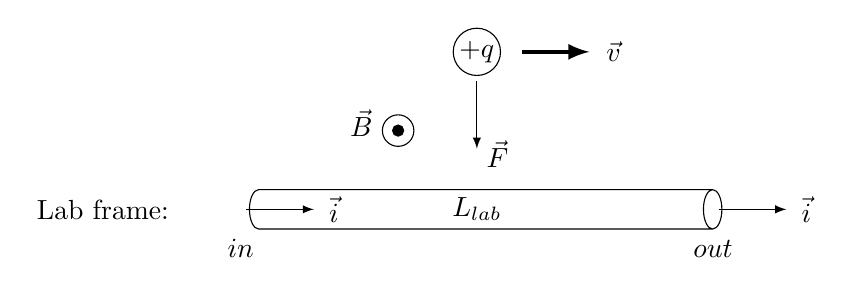
\begin{tikzpicture}[>=latex,shorten >=2pt,shorten <=2pt,shape aspect=1]
	
		%velocity vector
		\draw[->, ultra thick](0.5,2)--(1.5,2) node[right] {$\vec{v}$};
	
		%\charged particle
		\draw (0,2) circle [radius=0.3] node {$+q$}; 
 		
 		%conductor 1
 		\node at (-4.75,-0.25) [above] {Lab frame:};
 		\node at (0,0)[cylinder, shape border rotate=0, draw,minimum height=6cm,minimum width=0.5cm]{};
 		\node at (0,0) {$L_{lab}$};
 		\node at (3,-0.5) {$out$};
 		\node at (-3,-0.5) {$in$};
 		
 		%current arrow
 		\draw[->] (-3,0) -- (-2,0) node[right] {$\vec{i}$};
 		\draw[->] (3,0) -- (4,0) node[right] {$\vec{i}$};
 		
 		%magnetic field
 		\draw [fill=black,yshift=1cm,xshift=-1cm] circle (2pt) node [left] {};
 		\node at (-1.2,1.1) [left] {$\vec{B}$};
 		\draw (-1,1) circle [radius=0.2] node {$\dotfill$};
 		
 		%force vector
 		\draw[->] (0,1.7)--(0,0.7) node[right]{$\vec{F}$};
 		
	\end{tikzpicture}
 	\caption{Lab frame: EM and Relativity "experimental" setup}
 	\label{fig: lab frame}
 \end{figure}
 \noindent Recall the expression for the magnitude of the magnetic field as a function of distance from a long, thin conductor with current $\vec{i}$:
 \begin{equation}\label{eq:4.5}
 ||\vec{B}||=\frac{\mu_{0} i}{2\pi r}
 \end{equation}
 \noindent Note that the only force acting the charged particle is the Lorentz force because the conductor, while contains a current, is neutral: $q_{in} = q_{out}$. Hence, from \eqref{eq:4.6}, working the lab frame, we can write down the expression for the magnitude of the Lorentz force acting on the particle:
 \begin{equation}\label{eq:4.6}
 ||\vec{F}_{Lorentz}||=q||\vec{v}\cross\vec{B}||=\frac{qv\mu_{0} i}{2\pi r}
 \end{equation}
 \noindent The next step is to teleport ourselves into the particle's frame. As a result, the particle is now at rest while the conductor and the current inside the conductor move in the opposite direction. 
 \begin{figure}[!htb]
 	\centering
 	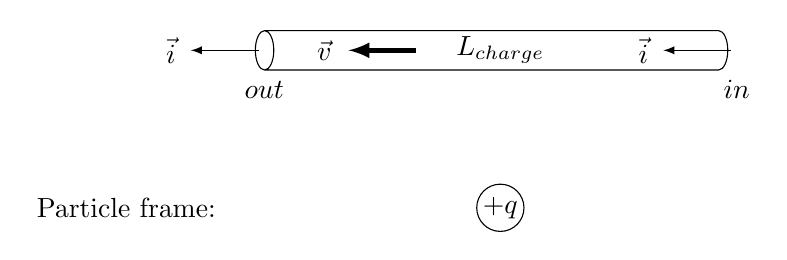
\begin{tikzpicture}[>=latex,shorten >=2pt,shorten <=2pt,shape aspect=1]
 	
 	%velocity vector
 	\draw[->, ultra thick](-1,2)--(-2,2) node[left] {$\vec{v}$};
 	
 	%\charged particle
 	\draw (0,0) circle [radius=0.3] node {$+q$}; 
 	
 	%conductor 1
 	\node at (-4.75,-0.25) [above] {Particle frame:};
 	\node at (0,2)[cylinder, shape border rotate=180, draw,minimum height=6cm,minimum width=0.5cm]{};
 	\node at (0,2) {$L_{charge}$};
 	\node at (-3,1.5) {$out$};
 	\node at (3,1.5) {$in$};
 	
 	%current arrow
 	\draw[->] (-3,2) -- (-4,2) node[left] {$\vec{i}$};
 	\draw[->] (3,2) -- (2,2) node[left] {$\vec{i}$};
 	
 	%magnetic field
 	%\draw [fill=black,yshift=1cm,xshift=-1cm] circle (2pt) node [left] {};
 	%\node at (-1.2,1.1) [left] {$\vec{B}$};
 	%\draw (-1,1) circle [radius=0.2] node {$\dotfill$};
 	
 	%force vector
 	%\draw[->] (0,1.7)--(0,0.7) node[right]{$\vec{F}$};
 	
 	\end{tikzpicture}
 	\caption{Particle frame: EM and Relativity "experimental" setup}
 	\label{charge frame}
 \end{figure}

 \noindent What's happening here is quite different from the previous scenario. The conductor in this case is no longer neutral because of the \textbf{rear clock ahead} effect. Precisely speaking, in the particle's frame, there is a net charge in the conductor at any given length $L_{charge}$ because the particle always sees charges coming into the conductor \textbf{before} it sees charges leave. Therefore, $q_{in} > q_{out}$. There exists a net charge, and we should be able to work out how much net charge there is.\\
 First, based on the \textbf{rear clock ahead} effect, working in the frame of the charged particle, we know the time difference $\Delta t^{\prime}$ between when charges come in and when charges come out of the conductor:
 \begin{equation} \label{eq:4.7}
 \Delta t^{\prime}=\frac{vL_{charge}}{c^2}=\frac{L^{\prime}v}{c^2}
 \end{equation}
 where $L_{charge}=L^{\prime}$ is the length of the conductor in the $+q$ particle's frame.\\ 
 \noindent So the net charge $q'$ on the conductor, in the particle's frame is
 \begin{equation} \label{eq:4.8}
 q^{\prime}=i\Delta t^{\prime}=i\frac{L^{\prime}v}{c^2}
 \end{equation}
 Our goal is to find the electric force acting on the charged particle from a charged, long, thin conductor. Recall the expression for the electric field from a line of charge:
 \begin{equation} \label{eq:4.9}
 E=\frac{1}{2\pi\epsilon_{0}}\frac{\lambda}{r}
 \end{equation}
 where $r$ is the distance from the particle to the conductor, and $\lambda=\frac{q'}{L'}$ is the conductor's linear charge density. \\
 Combining this expression with \eqref{eq:4.7} and \eqref{eq:4.8},
 \begin{equation} \label{eq:4.10}
 E=\frac{1}{2\pi\epsilon_{0}}\frac{\lambda}{r}=\frac{1}{2\pi\epsilon_{0}}\frac{1}{r}\frac{q'}{L'}=\frac{1}{2\pi\epsilon_{0}}\frac{iv}{rc^2}
 \end{equation}
 Hence, the electric force acting on the charged particle is
 \begin{equation}\label{eq:4.11}
 F_{q}=qE=\frac{q}{2\pi\epsilon_{0}}\frac{iv}{rc^2}
 \end{equation}
 Now, recall the relation between the speed of light $c$ and $\mu_{0}$ and $\epsilon_{0}$.
 \begin{equation}\label{eq:4.12}
 c=\frac{1}{\sqrt{\mu_{0}\epsilon_{0}}}
 \end{equation}
 So \eqref{eq:4.11} is essentially \eqref{eq:4.6}
 \begin{equation}\label{4.13}
 F_{q}=qE=\frac{q}{2\pi\epsilon_{0}}\frac{iv}{rc^2}=\frac{qv\mu_{0} i}{2\pi r}
 \end{equation}
 
 \subsubsection{Simultaneity and relativity: A cautionary tale}
 %some more math
 % another clock reading diagram
 So far, we have mostly worked in Bob's frame, deriving expressions for time differences in her frame. We have come to a conclusion that simultaneous events in Bob's frames are not necessarily simultaneous in Alice's frame. We have also found that while Alice and Bob both have synchronized clocks in their respective frames, Bob perceives Alice's rear clocks to have higher readings than her front clocks do. The next question we will be trying to answer, working in Bob's frame is: What readings does Alice see on Bob's clock if events are simultaneous in Alice's frame? To answer this question, we will briefly take a look at an old example involving some spacetime diagrams. Our goal is to write the expression for the time difference in Bob's frame (the ground frame), if events are simultaneous in Alice's frame. Since Alice is moving to the ``right'' of Bob, in Alice's frame, Bob is moving to the ``left'' of Alice. We obtain the two following spacetime diagrams.
 
 \begin{figure}[!htb] %place figure here
 	\centering
 	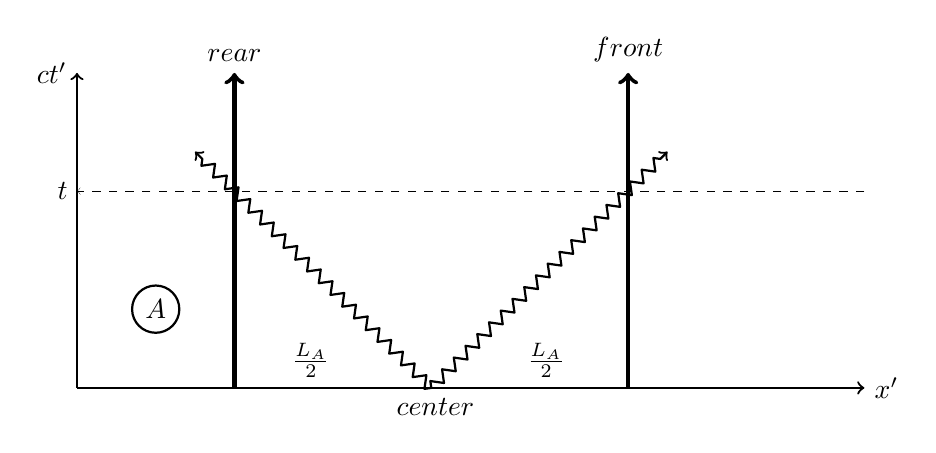
\begin{tikzpicture}[->, thick]
 	\draw (0,0,0) -- (0,4,0) node[left] {$ct'$}; %+Y
 	\draw [ultra thick](2,0,0) -- (2,4,0) node[above] {$rear$}; %+y'
 	\draw [ultra thick](7,0,0) -- (7,4,0) node[above] {$front$}; %+y'
 	
 	%horizontal axis
 	\draw (0,0,0) -- (10,0,0) node[right] {$x'$} node[above, xshift=-200] {$\frac{L_{A}}{2}$} node[above, xshift=-115]{$\frac{L_{A}}{2}$} node[below, xshift=-155]{$center$}; %+x'
 	
 	
 	\draw [dashed, ultra thin] (10,2.5) -- (0,2.5,0) node[left]{$t$}; %+x---
 	
 	% light arrows
 	\draw [->, line join=round, decorate, decoration={zigzag, segment length=6, amplitude=2,post=lineto, post length=2pt}] (4.5,0) -- (1.5,3);
 	\draw [->, line join=round, decorate, decoration={zigzag, segment length=6, amplitude=2,post=lineto, post length=2pt}] (4.5,0) -- (7.5,3);
 	
 	%Alice's name:
 	\draw (1,1) circle [radius=0.3] node {$A$};
 	
 	\end{tikzpicture}
 	\caption{Alice's spacetime diagram, simultaneous events}
 	\label{fig: alice's spacetime 3}
 \end{figure}
 
 \begin{figure}[!htb] %place figure here
 	\centering
 	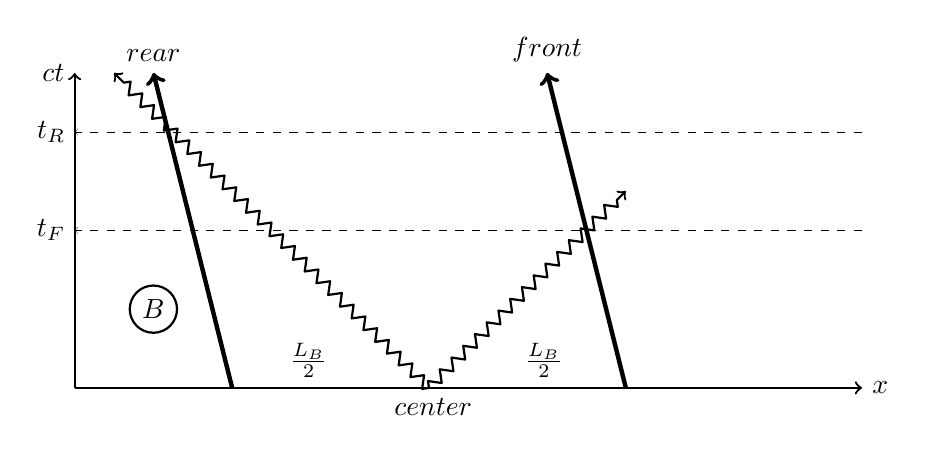
\begin{tikzpicture}[->, thick]
 	\draw (0,0,0) -- (0,4,0) node[left] {$ct$}; %+Y
 	\draw [ultra thick](2,0,0) -- (1,4,0) node[above] {$rear$}; %+y'
 	\draw [ultra thick](7,0,0) -- (6,4,0) node[above] {$front$}; %+y'
 	
 	\draw (0,0,0) -- (10,0,0) node[right] {$x$} node[above, xshift=-200] {$\frac{L_{B}}{2}$} node[above, xshift=-115]{$\frac{L_{B}}{2}$} node[below, xshift=-155]{$center$}; %+x
 	
 	\draw [dashed, ultra thin] (10,2) -- (0,2) node[left]{$t_{F}$}; %+x---
 	\draw [dashed, ultra thin] (10,3.25) -- (0,3.25) node[left]{$t_{R}$}; %+x---
 	
 	% light arrows
 	\draw [->, line join=round, decorate, decoration={zigzag, segment length=6, amplitude=2,post=lineto, post length=2pt}] (4.5,0) -- (0.5,4);
 	\draw [->, line join=round, decorate, decoration={zigzag, segment length=6, amplitude=2,post=lineto, post length=2pt}] (4.5,0) -- (7,2.5);
 	
 	%Bob's name:
 	\draw (1,1) circle [radius=0.3] node {$B$};
 	
 	\end{tikzpicture}
 	\caption{Bob's spacetime diagram, simultaneity in Alice's frame}
 	\label{fig: bob's spacetime 3}
 \end{figure} 
 
 \noindent Using our approach to the last example, we can quickly write down the expression for the time difference:
 
 \begin{equation}\label{eq:4.14}
 \Delta t_{B}=t_{R}-t_{F}=\frac{L_{B}}{2}\left(\frac{1}{c-v} - \frac{1}{c+v}\right) = \frac{L_{B}v}{c^2-v^2}=\frac{L_{B}v}{c^2}\left(\frac{1}{1-\frac{v^2}{c^2}}\right)
 \end{equation}
 At this point we must have seen this term $\frac{1}{1-v^2/c^2}$, or more precisely, its square root $\frac{1}{\sqrt{1-v^2/c^2}}$ enough times that we should assign to it a name. We shall be conventional and call this factor $\gamma$.
 \begin{equation}\label{eq:4.15}
 \Delta t_{B}=t_{R}-t_{F}=\frac{L_{B}v}{c^2}\left(\frac{1}{1-\frac{v^2}{c^2}}\right)=\frac{vL_{B}{\gamma}^{2}}{c^2}
 \end{equation}
 \noindent If we compare the form of \eqref{eq:4.15} to that of \eqref{eq:4.4}, we can see they differ by the square of factor $\gamma$. In the following sections, we will explore in more detail how the square of $\gamma$ comes to appear in \eqref{eq:4.15}, as well as its ubiquity and vital role in relativity. 
 
 \subsection{Relativity and how to understand space and time}
  So, just a recap, we shall review a few yet important rules to keep in mind when dealing with problems in special relativity:
  
 \textbf{First, all observers agree on events.} Recall our example of Alice and Bob. While they may disagree on the simultaneity of events, depending on their relative motions, they must and always agree that the light pulses arrive at the ends of the train. In same rule also applies to our previous example involving relativity and magnetism. Both the moving charged particle $+q$ and us agree that it is attracted to the conductor with current $i$. We should also extend beyond the scope of our examples. The order of events is also crucial in relativity. If, for instance, Alice calls and Bob responds, then regardless of which frame we are in (which results in certain time differences between the two events), we should never see the events in reverse orders, that is Bob responds \textbf{before} Alice calls. This is also known as the principle of causality.
 
 \textbf{Second, the principle of relativity and constancy of the speed of light.} Einstein's postulates are the foundation for all of our derivations. Indeed, without the assumption that all observers agree on the universal speed of light regardless of their reference frame, we would not be able to derive \textbf{rear clock ahead}, and different approaches to find the force on the charged particle will give different answer in different reference frames, which violate the first rule.
 
 \textbf{Third, all situations need to be measured with real tools: Sticks and Clocks.} Note that we abstain from using the phrase: ``Bob sees the light pulse arriving..." or "Alice sees Bob's clock readings..." This is intentional in order for an observer to ``see'' an event, light (or more precisely, information) from that event must reach the observer's eye, and then be processed by the brain... The point is that in special relativity, we often talk about measurements made in one frame or another, and these measurements are typically of ``time,'' which is given by clock readings, and ``location,'' which is given by the number of meter sticks. Our goal is to associate measurements with physical objects that belong to certain frames because as we will find out, one meter or one second in one frame are not necessarily the same in other frames. By knowing from which frames certain measurements are made and how these frames move relative to other frames, we can then ``convert'' these measurements between frames. 

 So, a quick recap on 3 important rules to keep in mind:
 
 - All observers agree on events.
 
 - The principle of relativity and constancy of the speed of light.
 
 - All situations need to be measured with real tools.
 
 In the following sections, we will be investigating other effects of special relativity. Specifically, we will explore how relative motions between different frames affect measurements of lengths and time intervals in another frame. In a physical sense, we are trying to answer questions like: ``How many meters is a meter in a moving frame?'' or ``How many seconds is a second in a moving frame?''
 \subsection{Transverse length measurements}
 First, we are interested in whether different observers agree on transverse lengths. Consider a thought experiment in which a cylinder of radius $r$ enters an annular cylinder with inner radius $r$ with velocity $\vec{v}$.
 \begin{figure}[!htb]
 	\centering
 	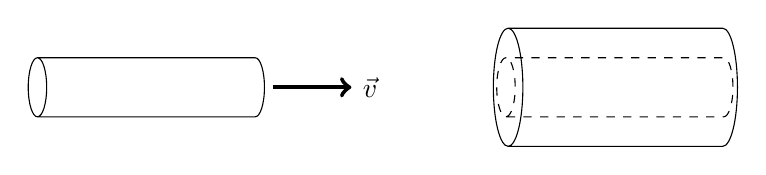
\begin{tikzpicture}
 	
 	%velocity vector
 	\draw[->, ultra thick](1.5,0)--(2.5,0) node[right] {$\vec{v}$};
 	
 	%cylinder 1
 	%\node at (-4.75,-0.25) [above] {Lab frame:};
 	\node at (0,0)[draw, cylinder, shape border rotate=180,minimum height=3cm,minimum width=0.75cm]{};
 	
 	%cylinder 2
 	\node at (5.95,0)[dashed, draw, cylinder, shape aspect = 1, shape border rotate=180, minimum height=3cm, minimum width=0.75cm]{};
 	\node at (6,0)[cylinder, draw, shape aspect = 1.6, shape border rotate=180, minimum height=3.1cm, minimum width=1.5cm]{};
 	
 	\end{tikzpicture}
 	\caption{Though experiment: Cylinders and transverse lengths}
 	\label{fig: transverse length thought experiment}
 \end{figure}
 
 \noindent We as observers are in the ground frame along with the annular cylinder. In our frame, the smaller cylinder is moving to the right with speed $v$. Three things can happen to transverse lengths (specifically radius $r$) of the smaller cylinder in our frame:
 
 - One, transverse lengths contract.
 
 - Two, transverse lengths expand.
 
 - Three, transverse lengths neither contract nor expand.
 
 \noindent Now, all observers, regardless of their reference frames, must agree that the cylinder has to fit the annular cylinder (because radius of the smaller cylinder is the same as the inner radius of the annular cylinder). Therefore, in our frame, the transverse lengths of the smaller cylinder must not expand. Thus, we rule out the second hypothesis. 
 
 \noindent The first hypothesis is a no more simple to rule out. Assume that transverse lengths in moving frames contract. Then if we out ourselves in the smaller cylinder's frame, we would measure the inner radius of the annular cylinder to be smaller than $r$, so the smaller cylinder does not fit inside the annular cylinder. This contradicts a point we made earlier about all observers must agree that the smaller cylinder can fit inside the annular cylinder. Hence, we rule out the first hypothesis.
 
 \noindent This leaves us with the only (and correct) hypothesis that transverse lengths neither expand nor contract. Based on the ``invariance'' of events, we have successfully argued that moving objects ``retain'' their stationary transverse dimensions. 
 
 \subsection{Time dilation}
 The next fundamental effect of relativity is \textbf{time dilation}, or ``moving clocks run slow.'' In order to demonstrate this effect and mathematically describe its consequences, we use a classic (thought) experiment which involves a light-pulse clock, Alice, Bob, and their respective trains.
 
 \begin{figure}[htb] 
 	\centering
 	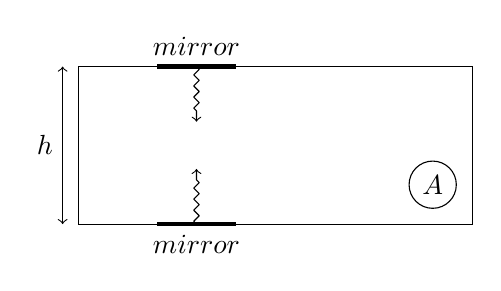
\begin{tikzpicture}
 	
 	%car
 	\draw (0,0)--(5,0)--(5,2)--(0,2)--cycle;
 	
 	%mirrors
 	\draw [ultra thick] (1,2)--(2,2) node[above, xshift=-0.5cm]{$mirror$};
 	\draw [ultra thick] (1,0)--(2,0) node[below, xshift=-0.5cm]{$mirror$};
 	
 	%light up
 	\draw [->, line join=round, decorate, decoration={zigzag, segment length=4, amplitude=1,post=lineto, post length=2pt}] (1.5,0) -- (1.5,0.7);
 	
 	%light down
 	\draw [->, line join=round, decorate, decoration={zigzag, segment length=4, amplitude=1,post=lineto, post length=2pt}] (1.5,2) -- (1.5,1.3);
 	
 	%height indicator
 	\draw [<->] (-0.2,0)--(-0.2,2) node[left, yshift=-1cm]{$h$};
 	
 	%Alice
 	\draw (4.5,0.5) circle [radius=0.3] node {$A$};
 	
 	\end{tikzpicture}
 	\caption{Light-clock experiment: Alice's frame}
 	\label{fig: alice's frame 2}
 \end{figure}
 \noindent A light-pulse clock in Alice's frame is shown in Figure \ref{fig: alice's frame 2}. The clock works by sending a pulse of light into a pair of mirrors, one placed on the floor of the train, the other on the ceiling, both aiming to keep light bouncing back-and-forth between themselves. Unlike regular clocks which ticks every second, the light-pulse clock ticks every time the pulse of light hits the bottom mirror. Given $c$ is the speed of light and $h$ is the height of the train, we obtain the tick-period of this clock, in Alice's frame
 \begin{equation}\label{eq:4.16}
 \tau_{A}=\frac{2h}{c}
 \end{equation}
 In Bob's frame, Alice (and her clock) is moving to the right with speed $v$. As we might expect, Bob sees things a little bit differently.
 \begin{figure}[htb] 
 	\centering
 	\begin{tikzpicture}
 	
 	%height indicator
 	\draw [<->] (5.2,0)--(5.2,2) node[right, yshift=-1cm]{$h$};
 	
 	%car1
 	\draw (0,0)--(5,0)--(5,2)--(0,2)--cycle node[left, yshift=1cm, xshift=-0.4cm]{$t=0$};
 	%mirrors1
 	\draw [ultra thick] (1,2)--(2,2);%top
 	\draw [ultra thick] (1,0)--(2,0);%bottom
 	%light up1
 	\draw [->, line join=round, decorate, decoration={zigzag, segment length=4, amplitude=1,post=lineto, post length=2pt}] (1.5,0) -- (1.7,0.7);
 	
 	%car2
 	\draw (0.5,-2.5)--(5.5,-2.5)--(5.5,-0.5)--(0.5,-0.5)--cycle node[left, yshift=1cm, xshift=-0.7cm]{$t=\frac{\tau_{B}}{2}$};
 	%mirrors2
 	\draw [ultra thick] (1.5,-0.5)--(2.5,-0.5);%top
 	\draw [ultra thick] (1.5,-2.5)--(2.5,-2.5);%bottom
 	%light down1
 	\draw [->, line join=round, decorate, decoration={zigzag, segment length=4, amplitude=1,post=lineto, post length=2pt}] (1.8,-1.2)--(2,-0.5) -- (2.2,-1.2);
 	
 	%car3
 	\draw (1,-5)--(6,-5)--(6,-3)--(1,-3)--cycle node[left, yshift=1cm, xshift=-1.2cm] {$t=\tau_{B}$};
 	%mirrors3
 	\draw [ultra thick] (2,-3)--(3,-3);%top
 	\draw [ultra thick] (2,-5)--(3,-5);%bottom
 	%light up3
 	\draw [->, line join=round, decorate, decoration={zigzag, segment length=4, amplitude=1,post=lineto, post length=2pt}] (2.3,-4.3)--(2.5,-5) -- (2.7,-4.3);
 	
 	%Bob and +y, t=0 line
 	\draw [dashed](0,1.3) -- (0,-5.2);
 	\draw [dashed](0,-2.5) -- (0.5,-2.5);
 	\draw [dashed](0,-5) -- (1,-5);
 	\draw (0,-5.5) circle [radius=0.3] node {$B$};
 	
 	%velocity vector
 	\draw [->, ultra thick] (4,2.5) -- (5,2.5) node[right] {\textbf{$\vec{v}$}};
 	
 	\end{tikzpicture}
 	\caption{Light-clock experiment: Bob's frame}
 	\label{fig: bob's frame 2}
 \end{figure}

 \noindent Our goal is to find $\tau_{B}$, which in this case is the time light takes to travel the diagonal path twice (up and down in Alice's train). We can approach this problem the same way we did in an earlier example with the Michelson-Morley interferometer. First, we can express the distance light travels in $\tau_{B}$. Note here that the train's height $h$ is retained. 
 \begin{equation}\label{eq:4.17}
 c\tau_{B}=2\sqrt{h^2 + {\left(\frac{v\tau_{B}}{2}\right)}^{2}}
 \end{equation}
 With some rearrangements, we obtain an expression for $\tau_{B}$:
 \begin{equation}\label{eq:4.18}
 \begin{split}
 \tau_{B}&=\sqrt{\frac{4h^2}{c^2-v^2}}\\
 &=\left(\frac{2h}{c}\right)\frac{1}{\sqrt{1-v^2/c^2}}\\
 &=\frac{2h\gamma}{c}
 \end{split}
 \end{equation}
 From \eqref{eq:4.16} and \eqref{eq:4.18}, we obtain a very important relation:
 \begin{equation}\label{eq:4.19}
 \tau_{B}=\gamma\tau_{A}
 \end{equation}
 
 \noindent This relation tells us that Bob would measure the tick-period of Alice's clock to be $\gamma$ times larger than the tick-period of the clock in Alice's frame. In other words, \textbf{in Bob's perspective, Alice's clock runs slow}. 
 
 \noindent It is also worth mentioning that the same logic can be applied to a different situation where Alice measures Bob's tick-period. Using the same derivation and setup, we should arrive at $\tau_{A} = \gamma\tau_{B}$. It can be tempting to think of this solution as paradoxical and contradictory to what we obtained earlier. However, if we think very carefully about how measurements are made, then there is no such paradox! Consider the diagram below, which represents a visual resolution to this apparent ``paradox.''
 
 \begin{figure}[!htb]
 	\centering
 	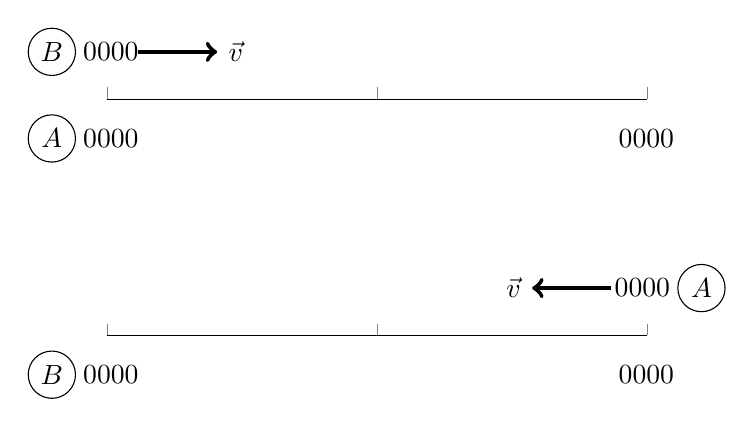
\begin{tikzpicture}
 	
 	%Alice's clocks
 	\node at (0.75,-0.5) {$\LARGE\showclock{00}{00}$};
 	%\node at (4.15,-0.5) {$\LARGE\showclock{00}{00}$};
 	\node at (7.55,-0.5) {$\LARGE\showclock{00}{00}$};
 	
 	%Bob's running clock
 	\node at (0.75,0.6) {$\LARGE\showclock{00}{00}$};
 	%Bob's clock velocity vector
 	\draw[->, ultra thick] (1.1,0.6)--(2.1,0.6) node[right]{$\vec{v}$};
 	
 	%Alice and Bob
 	\draw (0,-0.5) circle [radius=0.3] node {$A$}; 
 	\draw (0,0.6) circle [radius=0.3] node {$B$}; 
 	
 	\begin{axis}[y=1,xshift=20, hide y axis, axis x line*=bottom, xmin=0, xmax=10, xtick={0,5,10}, xticklabels=\empty]
 	\addplot [] table {
 		0 1
 		0 1
 	};
 	\end{axis}
 	
 	%Bob's clocks
 	\node at (0.75,-3.5) {$\LARGE\showclock{00}{00}$};
 	%\node at (4.15,-3.5) {$\LARGE\showclock{00}{00}$};
 	\node at (7.55,-3.5) {$\LARGE\showclock{00}{00}$};
 	
 	%Alice's running clock
 	\node at (7.5,-2.4) {$\LARGE\showclock{00}{00}$};
 	%Alice's clock velocity vector
 	\draw[->, ultra thick] (7.1,-2.4)--(6.1,-2.4) node[left]{$\vec{v}$};
 	
 	%Bob and Alice
 	\draw (8.25,-2.4) circle [radius=0.3] node {$A$};
 	\draw (0,-3.5) circle [radius=0.3] node {$B$};
 	
 	\begin{axis} [y=1,xshift=20, yshift=-3cm, hide y axis, axis x line*=bottom, xmin=0, xmax=10, xtick={0,5,10}, xticklabels=\empty]
 	\addplot [] table {
 		0 1
 		0 1
 	};
 	\end{axis}
 	\end{tikzpicture}
 	\caption{Resolution to time dilation ``paradox''}
 	\label{fig: time dilation resolution}
 \end{figure}
 \noindent Figure 23 aims to show an \textbf{asymmetry} in the comparison we are trying to make that leads to an apparent ``paradox.'' While Bob uses \textbf{his clocks} to measure Alice's time, Alice uses \textbf{her clocks} to measure Bob's time. And as we have found earlier, Alice and Bob do not always agree on their clock readings. Therefore, the statements "Alice's clocks run slow" or "Bob's clock run slow" are valid only if we also indicate the reference frames on which these statements are based. 
 
 \subsection{Length contraction}
 In this section we are going to explore the fourth and last fundamental effect of special relativity: \textbf{length contraction}. Using a similar setup as that in the previous section, except for the orientation of the light clock, we will find the relation between $L_{A}$ and $L_{B}$.
 \begin{figure}[htb] 
 	\centering
 	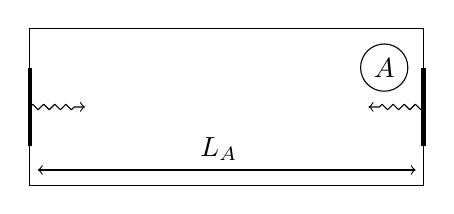
\begin{tikzpicture}
 	
 	%car
 	\draw (0,0)--(5,0)--(5,2)--(0,2)--cycle;
 	
 	%mirrors
 	\draw [ultra thick] (0,0.5)--(0,1.5);
 	\draw [ultra thick] (5,0.5)--(5,1.5);
 	
 	%light up
 	\draw [->, line join=round, decorate, decoration={zigzag, segment length=4, amplitude=1,post=lineto, post length=2pt}] (0,1) -- (0.7,1);
 	
 	%light down
 	\draw [->, line join=round, decorate, decoration={zigzag, segment length=4, amplitude=1,post=lineto, post length=2pt}] (5,1) -- (4.3,1);
 	
 	%length indicator
 	\draw [<->] (0.1,0.2)--(4.9,0.2) node[above, xshift=-2.5cm]{$L_{A}$};
 	
 	%Alice
 	\draw (4.5,1.5) circle [radius=0.3] node {$A$};
 	
 	\end{tikzpicture}
 	\caption{Light-clock experiment: Alice's frame}
 	\label{fig: alice's frame 3}
 \end{figure}
 Instead of sending vertical pulse, the light clock in this setup sends a pulse of light in the direction of motion. In Alice's frame, the tick-period is
 \begin{equation}\label{eq:4.20}
 {\tau_{A}}^{\prime}=\frac{2L_{A}}{c}
 \end{equation}
 \noindent where the prime is there just to help us distinguish the the longitudinal tick-period (which is what we are trying to find) from the vertical tick-period that we have found earlier. 
 
 \noindent In Bob's frame, the light pulses have to travel extra/less distances depending on their direction of motion. This is due to the rightward motion of Alice's frame with respect to the ground frame. 
 \begin{figure}[htb] 
 	\centering
 	\begin{tikzpicture}
 	
 	%length indicator
 	\draw [<->] (0.1,0.2)--(4.9,0.2) node[above, xshift=-2.5cm]{$L_{B}$};
 	
 	%car1
 	\draw (0,0)--(5,0)--(5,2)--(0,2)--cycle node[left, yshift=1cm, xshift=-0.4cm]{$t=0$};
 	%mirrors1
 	\draw [ultra thick] (0,0.5)--(0,1.5);%top
 	\draw [ultra thick] (5,0.5)--(5,1.5);%bottom
 	%light up1
 	\draw [->, line join=round, decorate, decoration={zigzag, segment length=4, amplitude=1,post=lineto, post length=2pt}] (0,1) -- (0.7,1);
 	
 	%car2
 	\draw (0.5,-2.5)--(5.5,-2.5)--(5.5,-0.5)--(0.5,-0.5)--cycle node[left, yshift=1cm, xshift=-0.7cm]{$t=\frac{{\tau_{B}}^{\prime}}{2}$};
 	%mirrors2
 	\draw [ultra thick] (0.5,-2)--(0.5,-1);%top
 	\draw [ultra thick] (5.5,-2)--(5.5,-1);%bottom
 	%light down1
 	\draw [->, line join=round, decorate, decoration={zigzag, segment length=4, amplitude=1,post=lineto, post length=2pt}] (5.5,-1.5) -- (4.8,-1.5);
 	
 	%car3
 	\draw (1,-5)--(6,-5)--(6,-3)--(1,-3)--cycle node[left, yshift=1cm, xshift=-1.2cm] {$t={\tau_{B}}^{\prime}$};
 	%mirrors3
 	\draw [ultra thick] (1,-4.5)--(1,-3.5);%top
 	\draw [ultra thick] (6,-4.5)--(6,-3.5);%bottom
 	%light up3
 	\draw [->, line join=round, decorate, decoration={zigzag, segment length=4, amplitude=1,post=lineto, post length=2pt}] (1,-4) -- (1.7,-4);
 	
 	%Bob and +y, t=0 line
 	\draw [dashed](0,1.3) -- (0,-5.2);
 	\draw [dashed](0,-2.5) -- (0.5,-2.5);
 	\draw [dashed](0,-5) -- (1,-5);
 	\draw (0,-5.5) circle [radius=0.3] node {$B$};
 	
 	%velocity vector
 	\draw [->, ultra thick] (4,2.5) -- (5,2.5) node[right] {\textbf{$\vec{v}$}};
 	
 	\end{tikzpicture}
 	\caption{Light-clock experiment: Bob's frame}
 	\label{fig: bob's frame 3}
 \end{figure}

 \noindent Similar to what we did in the previous section, we can set up an equation to solve for ${\tau_{B}}^{\prime}$
 \begin{equation}\label{eq:4.21}
 {\tau_{B}}^{\prime}=\frac{L_{B}}{c+v}+\frac{L_{B}}{c-v}=\frac{2L_{B}c}{c^2-v^2}=\left(\frac{2L_{B}}{c}\right)\frac{1}{1-v^2/c^2}=\frac{2L_{B}}{c}{\gamma}^{2}
 \end{equation}
 From \eqref{eq:4.19}, we know that ${\tau_{B}}^{\prime}=\gamma{\tau_{A}}^{\prime}$. So from \eqref{eq:4.20} and \eqref{eq:4.21}, we get the relation between length measurements between relatively moving frames:
 \begin{equation}\label{eq:4.22}
 L_{B}=\frac{L_{A}}{\gamma}
 \end{equation}
 
 \noindent This relation tells us that Alice's (longitudinal) lengths appear to be $\gamma$ times smaller in Bob's frame. Hence we call this effect \textbf{length contraction}. Note that Alice would also measure longitudinal lengths in Bob's frame to be $\gamma$ times smaller than their lengths in Bob's frame. While these (true) statements seem paradoxical, recall the argument we made about \textbf{asymmetrical} comparisons. Both Alice and Bob measure the other's longitudinal lengths as contracted. But this is totally fine (no physics is violated here) because both are in different point of view. Special relativity is all about perspectives\textemdash frames of reference.  
 \subsection{Reflection on fundamental effects}
 So, just a quick recap on the basic idea\textemdash the one single cause of all fundamental effects of special relativity. We have found that clocks are out-of-sync between relatively moving frames. We have found that clocks in moving frames run slow. We have also found that objects shrink in their direction of motion. We should ask ourselves: ``What is the one cause of all these phenomena?'' The answer is \textbf{perspective}.
 
 \noindent In the following two subsections, we shall both test and apply the fundamental effects of special relativity to derive and make predictions of other consequences of relativity. In the first subsection, we will first look at a different approach to derive time dilation, using a regular clock instead of a light clock. Then, we will check for consistency among time dilation, length contraction, and rear clock ahead by deriving length contraction from the two other fundamental effects. In the second subsection, we will use the known fundamental effects to explore how we can convert measurements of velocities from one frame to another. 
 
 \subsubsection{Time dilation with regular clocks}
 We shall attempt to derive time dilation in a more practical manner (by which I mean clock that does not require a single pulse of light to bounce indefinitely many times between two mirrors): by using a clock that sends out radio pulses every $\tau$ seconds in its rest frame. Now, we assume that this clock ticks with period $g_{v}\tau$ and is moving \textbf{away} from us, the observers, at speed $v$. Let $f_{v}\tau$ denotes the period which we \textbf{detect} the pulses. Since following every tick, the clock moves an extra distance $c\Delta t=vg_{v}\tau$ to get to us, we get an expression for $f_{v}\tau$:
 \begin{equation}\label{eq:4.23}
 f_{v}\tau=g_{v}\tau + \frac{v}{c}g_{v}\tau
 \end{equation}
 Hence,
 \begin{equation}\label{eq:4.24}
 f_{v}=g_{v}\left(1+\frac{v}{c}\right)
 \end{equation}
 
 \noindent If the clock moves \textbf{towards} us, then we get an expression for $f_{-v}\tau$
 \begin{equation}\label{eq:4.25}
 f_{-v}\tau=g_{v}\tau - \frac{v}{c}g_{v}\tau
 \end{equation}
 which gives
 \begin{equation}\label{eq:4.26}
 f_{-v}=g_{v}\left(1-\frac{v}{c}\right)
 \end{equation}
 \noindent In the trivial case in which the clock is at rest, we would detect the pulses coming with period $\tau$. Our goal now is to relate $f_{v}$, $f_{-v}$, and $g_{v}$ in a way such that we can express $g_{v}$ in terms of $v$ and show how $\tau$ depends on $g_{v}$. In order to do so, we shall consider the following scenario: 
 \begin{figure}[!htb]
 	\centering
 	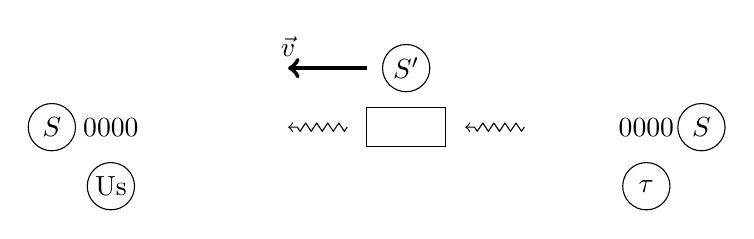
\begin{tikzpicture}
 	
 	%spaceship
 	\draw (4,-0.25)--(5,-0.25)--(5,0.25)--(4,0.25)--cycle node[]{};
 	
 	%S' frame
 	\draw (4.5,0.75) circle [radius=0.3] node {$S'$};
 	
 	%clocks
 	\node at (0.75,0) {$\LARGE\showclock{00}{00}$};
 	\node at (7.55,0) {$\LARGE\showclock{00}{00}$};
 	
 	%velocity vector
 	\draw[->, ultra thick] (4,0.75)--(3,0.75) node[above]{$\vec{v}$};
 	%\draw[dashed, ultra thin] (1.25,0)--(7,0);
 	
 	%S frame
 	\draw (0,0) circle [radius=0.3] node {$S$}; 
 	\draw (8.25,0) circle [radius=0.3] node {$S$};
 	\draw (7.55,-0.75) circle [radius=0.3] node {$\tau$}; 
 	\draw (0.75,-0.75) circle [radius=0.3] node {Us};
 	
 	%light pulses
 	\draw [->, line join=round, decorate, decoration={zigzag, segment length=4, amplitude=1.5,post=lineto, post length=2pt}] (6,0)--(5.25,0);
 	\draw [->, line join=round, decorate, decoration={zigzag, segment length=4, amplitude=1.5,post=lineto, post length=2pt}] (3.75,0)--(3,0);
 	
 	\end{tikzpicture}
 	\caption{Time dilation from a regular clock}
 	\label{fig: Time dilation from regular clock}
 \end{figure}
 
 \noindent The light clock with period $\tau$ is in the ground frame, but at some distance away from us. Now, a spaceship is traveling from the light clock towards us at speed $v$. Its job is to receive the light pulses from the clock and \textbf{instantaneously} transmit the pulse towards us (so the pulse is not interrupted). Since the spaceship is moving with speed $v$ away from the clock, it \textbf{sees} the pulses with period $f_{v}\tau$. Therefore, it also transmit at period $f_{v}\tau$. As a result, we (the ground frame) receives the pulses from the ship (which is moving towards us) at period $f_{-v}f_{v}\tau$. However, at the same time, we must see the light coming from the stationary clock period $\tau$ because the pulses are not delayed at the spaceship. Hence, we obtain an equation:
 \begin{equation}\label{eq:4.27}
 \tau=f_{-v}f_{v}\tau
 \end{equation}
 Therefore,
 \begin{equation}\label{eq:4.28}
 f_{-v}f_{v}={g_{v}}^{2}\left(1-\frac{v}{c}\right)\left(1+\frac{v}{c}\right)=1
 \end{equation}
 Following some rearrangements, we obtain this familiar expression for $g_{v}$:
 \begin{equation}\label{eq:4.29}
 g_{v}=\sqrt{\frac{1}{1-v^2/c^2}}
 \end{equation}
 Indeed, $g_{v}=\gamma$. So we can conclude clocks run slow in moving frames:
 \begin{equation}\label{eq:4.30}
 \tau_{v}=\gamma\tau_{0}
 \end{equation}
 \noindent At this point, we might be tempted to ask ourselves whether time dilation has ever been observed before\textemdash whether time dilation is \textbf{real}. And the answer is yes! In fact, the only reason we can detect large numbers (or any number at all) of muon particles $\mu^{-}$ from outer space at very low altitudes on Earth is due solely to time dilation. 
 
 \noindent Muons are subatomic particles that are very much similar to the electrons except for their greater mass and incredibly short half-life\textemdash approximately $150\mu s$. As these particles enter Earth's atmosphere, they enter at relativistic speeds close to the speed of light. Hence, despite their short lifetime, some muons indeed survive their entry to Earth and trigger ground detectors. What is so fascinating about the detection of muon particles, however, is the fact that they are detected in large numbers. At $2000m$, there are approximately $570{\mu}^{-}/hr$. Given their velocities and decay rate (which is found experimentally using particle accelerator), it is expected that at $50m$ above ground there should be less than $50{\mu}^{-}/hr$. In reality, however, scientists detected around $400{\mu}^{-}/hr$, significantly greater than the value predicted by our non-relativistic hypothesis.  
 
 \noindent We are certainly not so much puzzled by this fact because we have been equipped with the knowledge of time dilation. Muons are moving towards us with great (and by great I mean relativistic) speeds, thus their ``clocks,'' as seen from our frame, run slow. As a result, in our frame, these muons take longer than $150\mu s$ to decay and therefore are more likely to travel further down towards Earth. In their rest frame, however, a muon's half-life is still $150\mu s$. 
 
 \subsubsection{Length contraction revisited}
 Before moving on to the next subsection, we shall take a look back at the fundamental effects of special relativity\textemdash especially to check their consistency with each other. In this section, we will derive (yet again) length contraction, not using a light clock, but from rear clock ahead and time dilation. If our derivation leads us to the same conclusion we made about length contraction, then we can be confident that special relativity works (at least so far).
 
 \subsubsection{Velocity ``addition''}
 In this subsection we explore how velocities change as we move from one frame to another. At the moment, we have known that Alice and Bob disagree on their measurements of distances and time intervals, so it is reasonable to be careful about their agreement on velocities\textemdash the change of distance over time.
 
 \noindent Specifically, we are interested in how Alice's measurements of velocities change as we move from her frame to Bob's frame. Our goal is to setup an experiment in which a particle moves with speed $u^{\prime}$ in Alice's frame and apply our knowledge of the fundamental effects of special relativity (time dilation, length contraction, read clock ahead) to (hopefully) derive an expression for the speed $u$ of the same particle in Bob's frame, in relation to $u^{\prime}$. 
 
 \noindent Consider two events: a ball (1) leaving the rear of a train, and (2) arriving at the front of the train. In Alice's frame, she measures $\Delta x' = L_A$ as the distance the ball traverses and $\Delta t'$ as the time between these two events. In Bob's frame, he measures $\Delta x = L_B$ and $\Delta t$. Let us define $u' = \Delta x' / \Delta t'$ as the ball's velocity in Alice's frame, and $u = \Delta x / \Delta t$ as the ball's velocity in Bob's. The train is stationary in Bob's frame and is moving at speed $v$ in Alice's frame. Hence:
 
 \begin{equation}
 \Delta t' = \frac{L_A}{u'},
 \end{equation}
 and
 \begin{equation}
 \Delta t = \frac{L_B}{u - v}
 \end{equation}
 Working in Bob's frame, from length contraction, we know that:
 \begin{equation}
 L_B=\frac{L_A}{\gamma}=\frac{L_A}{\sqrt{1-v^2/c^2}}.
 \end{equation}
 And from time dilation and loss of simultaneity:  
 \begin{equation}
 \Delta t=(t_2-t_1)= \gamma \Delta t' = \gamma(t_2'-t_1')=\gamma\left(\frac{L_A}{u'} + \frac{L_A v}{c^2}\right). 
 \end{equation}
 From 4.31 to 4.34, we get:
 \begin{equation}
 \begin{split} 
 &\gamma\left(\frac{L_A}{u'} + \frac{L_A v}{c^2}\right) = \frac{L_A}{\gamma (u-v)} \\
 \therefore{}&\gamma\left( \frac{1}{u'} + \frac{v}{c^2} \right) = \frac{1}{\gamma (u-v)} \\
 \therefore{}& \frac{c^2-u'v}{u'c^2}=\frac{1}{\gamma^2}.\frac{1}{u-v}=\left(1-\frac{v^2}{c^2} \right).\frac{1}{u-v} \\
 \therefore{}&(c^2-u'v)(u-v)=(u'c^2)\left(1-\frac{v^2}{c^2} \right)\\
 \therefore{}&\dots\\
 \therefore{}&u'=\frac{u-v}{1-\frac{uv}{c^2}},
 \end{split}
 \end{equation}
 which is the expression for the ball's velocity in Alice's frame, working in Bob's frame.
 
 \noindent Similarly, working in Alice's frame:
 \begin{equation}
 u=\frac{u'+v}{1+\frac{u'v}{c^2}}.
 \end{equation}
 
 \noindent So far we have focused on deriving the expressions for velocity addition; however, the larger and more important point to note here is that velocities can never exceed $c$ the speed of light regardless of where the observation takes place. 
 
 \noindent For example, let Bob be in a stationary frame. Alice is moving relative to Bob at speed $0.9c$, and a ball is also moving at speed $0.9c$ in Alice's frame. Without any knowledge of special relativity, one might say the speed of the ball in Bob's frame is $u = 0.9c + 0.9c = 1.8c$. However, with velocity addition:
 \begin{equation}
 u = \frac{u'+v}{1+\frac{u'v}{c^2}} = \frac{1.80c}{1+\frac{0.81c^2}{c^2}} \approx 0.9945c < c.
 \end{equation}
 If $u'=c$, then:
 \begin{equation}
 u=\frac{c+u}{1+\frac{cv}{c^2}}=\frac{c(1+v/c)}{1+v/c}=c.
 \end{equation}
 What if $u'=0$?
 \begin{equation}
 u=\frac{v}{1+0}=v.
 \end{equation}
 Both of these two extreme cases make sense. 
 
 \newpage
 
 \section{Lorentz-Einstein Transformation Equations}
 In previous sections, we have derived expressions for time and spatial quantities of the same events in different frames. However, just in case you haven't noticed by now, going between frames can get quite cumbersome. 
 
 \noindent The goal of this section is to formulate a way to transform spatial and time coordinates from one frame to another. The Lorentz-Einstein transformation equations will be our tool. 
 
 \subsection{Linear transformation of coordinates}
 Let us define a set of equations which transform time and spatial coordinates in Bob's frame $(t,x,y,z)_S$ into Alice's frame $(t',x',y',z')_{S'}$:
 \begin{equation}
 \begin{split}
 x'&=a_{11}x + a_{12}y + a_{13}z + a_{14}t \\
 y'&=a_{21}x + a_{22}y + a_{23}z + a_{24}t \\
 z'&=a_{31}x + a_{32}y + a_{33}z + a_{34}t \\
 t'&=a_{41}x + a_{42}y + a_{43}z + a_{44}t 
 \end{split}
 \end{equation}
 
 \noindent We can write these equations in a form of a matrix equation:
 \begin{gather}
 \begin{bmatrix} x' \\ y' \\ z' \\ t' \end{bmatrix}
 =
 \begin{bmatrix}
 a_{11} & a_{12} & a_{13} & a_{14}\\
 a_{21} & a_{22} & a_{23} & a_{24}\\
 a_{31} & a_{32} & a_{33} & a_{34}\\
 a_{41} & a_{42} & a_{43} & a_{44}
 \end{bmatrix}
 \begin{bmatrix}
 x \\ y \\ z \\ t
 \end{bmatrix},
 \end{gather}
 just to emphasize a point that the Lorentz-Einstein equations make a ``linear transformation.'' Our goal is to figure out what the matrix elements are. 

 \subsection{Derivations}
 \subsubsection{Transverse dimension}
 Let us revisit the thought experiment in 4.3 where a solid cylinder of radius $r$ and length $l$ travels at speed $v$ and fits into a (stationary) annular cylinder of inner radius $r$ and length $l$. (Note: all lengths are lengths) measured in the rest frame).
 
  \begin{figure}[!htb]
 	\centering
 	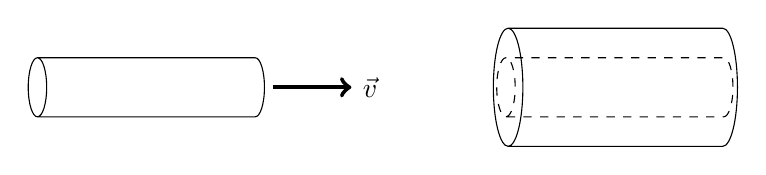
\begin{tikzpicture}
 	
 	%velocity vector
 	\draw[->, ultra thick](1.5,0)--(2.5,0) node[right] {$\vec{v}$};
 	
 	%cylinder 1
 	%\node at (-4.75,-0.25) [above] {Lab frame:};
 	\node at (0,0)[draw, cylinder, shape border rotate=180,minimum height=3cm,minimum width=0.75cm]{};
 	
 	%cylinder 2
 	\node at (5.95,0)[dashed, draw, cylinder, shape aspect = 1, shape border rotate=180, minimum height=3cm, minimum width=0.75cm]{};
 	\node at (6,0)[cylinder, draw, shape aspect = 1.6, shape border rotate=180, minimum height=3.1cm, minimum width=1.5cm]{};
 	
 	\end{tikzpicture}
 	\caption{Though experiment: Cylinders and transverse lengths}
 	\label{fig: transverse length thought experiment revisited}
 \end{figure}

 \noindent We have argued in 4.3 that since observers have to agree on \underline{events}, observers agree on the transverse lengths $y$ and $z$. So Eq. 5.2 becomes:
 
 \begin{equation}
 \begin{split}
 x'&=a_{11}x + a_{12}y + a_{13}z + a_{14}t \\
 y'&=y \\
 z'&=z \\
 t'&=a_{41}x + a_{42}y + a_{43}z + a_{44}t 
 \end{split}
 \end{equation}
 
 \noindent And the matrix equation becomes:
 \begin{gather}
 \begin{bmatrix} x' \\ y' \\ z' \\ t' \end{bmatrix}
 =
 \begin{bmatrix}
 a_{11} & a_{12} & a_{13} & a_{14}\\
 0 & 1 & 0 & 0\\
 0 & 0 & 1 & 0\\
 a_{41} & a_{42} & a_{43} & a_{44}
 \end{bmatrix}
 \begin{bmatrix}
 x \\ y \\ z \\ t
 \end{bmatrix},
 \end{gather}
   
 \subsubsection{$x-t$ transformation}
 Since $x'$ and $t'$ cannot depend on $y$ and $z$: $$ a_{12} = a_{13} = a_{42} = a_{43} = 0,$$ our matrix equation reduces to:
 \begin{gather}
 \begin{bmatrix} x' \\ y' \\ z' \\ t' \end{bmatrix}
 =
 \begin{bmatrix}
 a_{11} & 0 & 0 & a_{14}\\
 0 & 1 & 0 & 0\\
 0 & 0 & 1 & 0\\
 a_{41} & 0 & 0 & a_{44}
 \end{bmatrix}
 \begin{bmatrix}
 x \\ y \\ z \\ t
 \end{bmatrix}.
 \end{gather}
 
 \subsubsection{Dependence of $x',t'$ on $x,t$}
 Now, we will break down the $x-t$ dependence on $x'-t'$, in three steps:
 
 \noindent 1/ \underline{Consider a pulse of light traveling in the +x-axis}\\ 
 Let $\lambda$ and $\mu$ be arbitrary constants such that:
 \begin{align*}
 \lambda(x-ct) &= (x' - ct') \\
 \mu(x+ct) &= (x' + ct')
 \end{align*}
 It follows that:
 \begin{align*}
 2ct' &= (\mu-\lambda)x + c(\mu+\lambda)t \\
 2x' &= (\mu+\lambda)x + c(\mu-\lambda)t.
 \end{align*}
 Let $a=(\mu+\lambda)/2$ and $b=(\lambda-\mu)/2$, we get:
 \begin{align}
 ct' &= -bx + act \\
 x' &= ax - bct.
 \end{align}
 
 \noindent 2/ \underline{Consider the motion of the origins of $S$ and $S'$}\\
 $x'=0$, so $avt-bct=0$. Eq. 5.6 and Eq. 5.7 become:
 \begin{align}
 ct' &= a[ct-(v/c)x]=a(ct-\beta x) \\
 x' &= a[x -(v/c)ct]=a(x-\beta ct).
 \end{align}
 
 \noindent So in matrix form:
 \begin{gather}
 \begin{bmatrix} x' \\ y' \\ z' \\ t' \end{bmatrix}
 =
 \begin{bmatrix}
 a & 0 & 0 & -a\beta c\\
 0 & 1 & 0 & 0\\
 0 & 0 & 1 & 0\\
 -a\beta/c & 0 & 0 & a
 \end{bmatrix}
 \begin{bmatrix}
 x \\ y \\ z \\ t
 \end{bmatrix}.
 \end{gather}
 
 \noindent 3/ \underline{Apply the principle of relativity}\\
 The next reasonable step is to find what $a$ is. Let us return to our classic thought experiment: Alice moving relative to Bob at speed $v$, both making measurements of a train of proper length $l_0$. 
 
 \noindent Let everyone be initially at rest. Since Alice and Bob both have to agree on the length of the train:
 
 \noindent - Working in $(S)$ (Bob's frame), at $t=0$: $x_L'=0$ and $x_R'=l_0$, where $x_L'$ is the position of the tail of the train, and $x_R'$ is the position of the head of the train in Alice's frame.  
 
 \noindent - Working in $(S')$ (Alice's frame), at $t'=0$: $x_L=0$ and $x_R=l_0$, where $x_L$ is the position of the tail of the train, and $x_R$ is the position of the head of the train in Bob's frame. 
 
 \noindent The question, then, is: ``In $(S')$, at $t'=0$, if $x_L'=0$ then what is $x_R'$?'' 
 
 \noindent To answer this question we use Eq. 5.8 and Eq. 5.9. Substituting the expression for $ct$ from Eq. 5.8 into Eq. 5.9, we get:
 \begin{equation}
 x_R'=a(x_R-\beta ct)=a\left[x_R-\frac{v}{c}\left(\frac{ct'}{a}+\frac{v}{c}x_R \right) \right].
 \end{equation}
 At $t'=0$, with $x_R'=l'$ and $x_R=0$, Eq. 5.11 simplifies to:
 \begin{equation}
 l'=al_0\left(1-\frac{v^2}{c^2} \right). 
 \end{equation}
 But we also know that at $t'=0$ (in Alice's frame, of course):
 \begin{equation}
 x_R'=ax_R \equiv l_0=al'.
 \end{equation}
 Combining Eq. 5.12 and 5.13:
 \begin{equation}
 \frac{l_0}{a}=al_0\left( 1-\frac{v^2}{c^2}\right). 
 \end{equation}
 Therefore:
 \begin{equation}
 a=\frac{1}{\sqrt{1-\frac{v^2}{c^2}}}=\gamma.
 \end{equation}
 Our matrix equation becomes:
 \begin{gather}
 \begin{bmatrix} x' \\ y' \\ z' \\ t' \end{bmatrix}
 =
 \begin{bmatrix}
 \gamma & 0 & 0 & -\gamma\beta c\\
 0 & 1 & 0 & 0\\
 0 & 0 & 1 & 0\\
 -\gamma\beta/c & 0 & 0 & \gamma
 \end{bmatrix}
 \begin{bmatrix}
 x \\ y \\ z \\ t
 \end{bmatrix}.
 \end{gather}
 We can tweak a little so that Eq. 5.16 looks more ``symmetric'' and conventional:
 \begin{gather}
 \begin{bmatrix} ct' \\ x' \\ y' \\ z' \end{bmatrix}
 =
 \begin{bmatrix}
 \gamma & -\beta\gamma & 0 & 0\\
 -\beta\gamma & \gamma & 0 & 0\\
 0 & 0 & 1 & 0\\
 0 & 0 & 0 & 1
 \end{bmatrix}
 \begin{bmatrix}
 ct \\x \\ y \\ z
 \end{bmatrix}.
 \end{gather}

 \subsection{The Lorentz-Einstein Equations}
 We can extract from Eq. 5.17 a set of equations called Lorentz-Einstein Equations.
 \begin{equation}
 \begin{cases}
 x'=\gamma(x-\beta ct)\\
 y'=y\\
 z'=z\\
 ct'=\gamma(ct-\beta x)
 \end{cases}
 \end{equation}
 Of course Eq. 5.17 and Eq. 5.18 are just different ways to express the same idea. Some may find the matrix equation more elegant and symmetric. Others may prefer the ``equations notation.'' At our level there is little advantage difference between the two expressions. 
 
 \subsection{Some properties of the Lorentz-Einstein Transformations}
 \subsubsection{Spatial separation and time interval between events}
 In $(S)$, let Event 1 be $(ct_1, x_1, y_1, z_1)_S$, and Event 2 be $(ct_2, x_2, y_2, z_2)_{S}$. (Recall that an ``Event'' can be represented by a set of spatial and time coordinates).
 
 \noindent The spatial separation of Event 2 and Event 1 in $(S)$ is:
 \begin{equation}
 \Delta x = x_2 - x_1.
 \end{equation} 
 
 \noindent The spatial separation of Event 2 and Event 1 in another frame $(S')$ is:
 \begin{equation}
 \begin{split}
 \Delta x' &= x_2' - x_1'\\
 &= \gamma(x_2-\beta\gamma t_2) - \gamma(x_1-\beta\gamma t_1)\\
 &= \gamma(x_2-x_1)-\gamma\beta c(t_2-t_1)\\
 &= \gamma(\Delta x - \beta c\Delta t).
 \end{split}
 \end{equation}
 Similarly, we can work out the time interval in $(S')$: 
 \begin{equation}
 \begin{split}
 c\Delta t' &= ct_2'-ct_1'\\
 &= \gamma(ct_2-\beta x_2) - \gamma(ct_1-\beta x_1)\\
 &= \gamma(c\Delta t - \beta\Delta x).
 \end{split}
 \end{equation}
 So spatial separations and time intervals transform like positions and time. 
 
 \subsubsection{Non-relativistic limit}
 As the ratio $v/c$ approaches 0, or analogously $c \rightarrow \infty$, $\gamma$ approaches 1:
 \begin{equation}
 \lim\limits_{c\rightarrow \infty} \gamma = 1.
 \end{equation} 
 At these limits, called ``non-relativistic`` limits, the Lorentz-Einstein Equations become:
 \begin{equation}
 \begin{cases}
 x'=x-vt\\
 y'=y\\
 z'=z\\
 t'=t
 \end{cases}
 \end{equation}
 which are nothing but the Galilean transformation equations that we are more familiar with. 
 \subsubsection{The limiting speed}
 The ubiquitous $\gamma$ factor plays a crucial role in coordinate transformations. 
 $$\gamma = \frac{1}{\sqrt{1-\frac{v^2}{c^2}}}.$$
 Intuitively, $\gamma$ represents how much time and space is stretched or contracted as we move between frames. However, the mathematical form of $\gamma$ places a limiting value on the speed $v$ in terms of the speed of light $c$.
 
 \noindent Specifically we observe that if $v=c$, then $\gamma \rightarrow \infty$, and if $v > s$ then $\gamma$ becomes imaginary. Therefore the speed of light $c$ is the limiting speed. Consequently no two frames can travel at $c$ relative to each other. In fact, no physical object (with non-zero mass) can travel at the speed of light or beyond.   
 \subsubsection{The limiting speed - REALLY!}
 Physics describes sequences of events that are \underline{causally related}. No matter in which reference frame observations are made, the law of physics (of our world at least) must retain the chronological order of events. The speed of light as the universal speed limit, which is the limiting speed of any signal of any type known or unknown, is placed under this assumption. 
 
 \noindent Let us imagine another thought experiment in which Event 1 $(ct_1,x_1)_S$ causes Event 2 $(ct_2,x_2)_S$ by sending a signal with speed $u_{Signal}$ through space. The spatial separation between the two Events in $(S)$ is:
 \begin{equation}
 \Delta x = x_2 - x_1 = u_{Signal}\Delta t. 
 \end{equation}
 In another reference frame $(S')$:
 \begin{equation}
 c\Delta t'=\gamma\left( c\Delta t - \frac{v}{c}\Delta x\right) =\gamma c\Delta t\left(1-\frac{v}{c^2}u_{Signal}\right).
 \end{equation}
 Since $\Delta t = t_2-t_1 > 0$ and $\gamma \geq 1$ (and $c>0$ of course), if $u_{Signal} > c$ then $\Delta t' < 0$. Therefore, if $u_{Signal} > c$ then there exists a frame $(S')$ with $v/c < 1$ in which the order of events 1 and 2 are reversed, violating causality. So if causality should never be violated, then $u_{Signal}$ must not exceed the speed of light $c$.
 
 \subsection{The fundamental effects and consequence of the Lorentz-Einstein transformation}
 Let us revisit the fundamental effects of special relativity (time dilation, length contraction, and loss of simultaneity) in the context of the Lorentz-Einstein Equations, which can be written in the matrix form as:
 \begin{gather*}
 \begin{bmatrix} ct' \\ x' \\ y' \\ z' \end{bmatrix}
 =
 \begin{bmatrix}
 \gamma & -\beta\gamma & 0 & 0\\
 -\beta\gamma & \gamma & 0 & 0\\
 0 & 0 & 1 & 0\\
 0 & 0 & 0 & 1
 \end{bmatrix}
 \begin{bmatrix}
 ct \\x \\ y \\ z
 \end{bmatrix}.
 \end{gather*}
 In this section we will re-derive/verify these effects, using the Lorentz-Einstein transformation equations.  
  
 \subsubsection{Time dilation}
 Consider a thought experiment in which a clock moves at speed $v$ relative to Bob (rest frame). At time $t_1$, the clock is at point $x_1$ in Bob's frame. We call this Event 1. At time $t_2$, the clock is at $x_2$. We call this Event 2. Alice also moves at the same speed $v$ relative to Bob. The clock is at rest in Alice's frame.
 
 \noindent Let Event 1 $(ct_1,x_1)$ and Event 2 $(ct_2, x_2)$ be given, then in $(S)$, let the spatial separation of these events be:
 \begin{equation}
 \Delta x = x_2-x_1=v\Delta t=v(t_2-t_1).
 \end{equation}
 In Alice's frame $(S')$, the spatial separation $\Delta x'$, according to the Lorentz-Einstein transformation equations, is:
 \begin{equation}
 \begin{split}
 \Delta x' &= \gamma(\Delta x-\beta c\Delta t)\\
 &= \gamma\left(\Delta x - \frac{v}{c}\frac{\Delta x}{v}c \right)\\
 &= 0, 
 \end{split}
 \end{equation}
 which makes sense because (again) the clock is at rest in Alice's frame. But what about the time interval between Event 2 and Event 1?
 
 \noindent In Alice's frame $(S')$:
 \begin{equation}
 \begin{split}
 c\Delta t' &= \gamma(c\Delta t-\beta\Delta x)\\
 &= \gamma \left(c\Delta t-\frac{v}{c}v\Delta t \right). 
 \end{split}
 \end{equation}
 Therefore, 
 \begin{equation}
 \begin{split}
 \Delta t'&=\gamma\left(\Delta t-\frac{v^2}{c^2}\Delta t \right) \\
 &= \gamma\Delta t\left(1-\frac{v^2}{c^2} \right) \\
 &= \gamma\Delta t\frac{1}{\gamma^2}\\
 &= \frac{\Delta t}{\gamma},
 \end{split}
 \end{equation}
 which is what ``time dilation'' means. 
 \subsubsection{Length contraction}
 Imagine a train at rest in Alice's frame, which is moving at speed $v$ relative to Bob. In Alice's frame, the train has length $l_0 = x_R'-x_L'=\Delta x'$. In Bob's frame, the length of the train is $l'=x_R-x_L=\Delta x$.
 
 \noindent According to the Lorentz-Einstein transformations:
 \begin{equation}
 \Delta x'=\gamma(\Delta x-\beta c \Delta t).
 \end{equation}  
 Since measurements are made simultaneously in Bob's frame, $\Delta t = 0$. Therefore Eq. 5.30 becomes:
 \begin{equation}
 \Delta x' = \gamma\Delta x.
 \end{equation}
 Or, equivalently:
 \begin{equation}
 l_0=\gamma l',
 \end{equation}
 which is what ``length contraction'' means. 
 
 \noindent We can, of course, derive the same result differently. Imagine if Bob measures the length of the train by measuring the time interval $\Delta t$ between the front and the back of the train passing through a point $x_0$ in Bob's frame. 
 
 \noindent According to Lorentz-Einstein equations, the length of the train in Alice's frame is:
 \begin{equation}
 \Delta x' = \gamma(\Delta x - \beta c \Delta t) = -l_0 = x_L'-x_R',
 \end{equation}
 note the minus sign represents how Bob's approach in making measurements is different than our previous approach. 
 
 \noindent Since Bob makes measurements at the same location, $\Delta x = 0$. From Eq. 5.33:
 \begin{equation}
 l_0 = \gamma \beta c \Delta t = \gamma c \left( \frac{v}{c}\right) \left( \frac{l'}{v}\right)  = \gamma l',
 \end{equation}
 which is the same result we obtained earlier. 
 
 \subsubsection{Relativity of simultaneity}
 We return to the question: ``If two events occur simultaneously in $(S)$ then what is the time interval between $(S')$?''
 
 \noindent According to the Lorentz-Einstein equations:
 \begin{equation}
 \begin{split}
 \Delta x' &= \gamma(\Delta x - \beta c \Delta t)\\
 c\Delta t' &= \gamma(c\Delta - \beta\Delta x ).
 \end{split}
 \end{equation}
 
 \noindent $\Delta t = 0$ since the two events occur simultaneously in $(S)$. From Eq. 5.35 we get the expression for the time interval in $(S')$:
 \begin{equation}
 \Delta t' = \frac{-\gamma\beta\Delta x}{c}=\frac{-v\Delta x'}{c^2},
 \end{equation}
 which is nothing but the ``rear-clock ahead'' effect.
 
 \newpage
 
 \section{Relativistic Kinematics: Motion of Particles}
 In this section we study how to describe the motions of particles in special relativity. Specifically, we study how to represent force, velocity, acceleration in space-time coordinates, as well as new kinetic effects that emerge as a result of relativity. 
 
 \noindent In previous sections, we have been studying how to transform spatial and time coordinates between frames: given $\left( x(t),y(t),z(t)\right) _S$, we can find $\left( x'(t'),y'(t'),z'(t')\right) _{S'}$. Now, the question simply becomes: given $\left(u_x(t),u_y(t), u_z(t) \right) _S$, can we find an expression for $\left( {u'}_{x'}(t'),{u'}_{y'}(t'),{u'}_{z'}(t')\right)_{S'}$? 
 
 \noindent While there are multiple ways to tackle this problem, one approach we will use here is the ``differential approach'' in which we convert finite intervals into differentials. What is means is to the bring the ``finite interval form'' of the Lorentz-Einstein equations that we are familiar with:
 \begin{equation}
 \begin{split}
 c\Delta t' &= \gamma(c\Delta t - \beta \Delta x) \\
 \Delta x' &= \gamma(\Delta x - \beta c \Delta t)\\
 \Delta y' &= \Delta y \\
 \Delta z' &= \Delta z
 \end{split}
 \end{equation}
 into ``differentials form:''
 \begin{equation}
 \begin{split}
 cdt' &= \gamma(cdt - \beta dx) \\
 dx' &= \gamma(dx - \beta c dt)\\
 dy' &= dy \\
 dz' &= dz.
 \end{split}
 \end{equation}
 \noindent Replacing $\beta c$ with $v$, which is the relative velocity between two reference frames, and $dx/dt$ with $u_x$:
 \begin{equation}
 \begin{split}
 cdt' &= \gamma\left( c - vu_x/c\right) dt \\
 dx' &= \gamma(u_x - v)dt\\
 dy' &= dy \\
 dz' &= dz.
 \end{split}
 \end{equation}
 
 \subsection{Longitudinal velocity transformation}
 From Eq. 6.3, we derive the expression for velocities in the longitudinal direction:
 \begin{equation}
 {u'}_x=\frac{dx'}{dt'}=\frac{u_x-v}{1-\frac{vu_x}{c^2}}.
 \end{equation}
 Inversely, 
 \begin{equation}
 {u}_x=\frac{dx}{dt}=\frac{{u'}_x+v}{1+\frac{v{u'}_x}{c^2}}.
 \end{equation}
 \subsection{Transverse velocity transformation}
 From Eq. 6.3, we derive the expression for velocities in the transverse direction:
 \begin{equation}
 {u'}_y=\frac{dy'}{dt'}=\frac{1}{\gamma\left( 1-\frac{vu_x}{c^2}\right) }\frac{dy}{dt} = \frac{u_y/\gamma}{1-\frac{vu_x}{c^2}}.
 \end{equation}
 Inversely,
 \begin{equation}
 u_y=\frac{{u'}_y/\gamma}{1+\frac{v{u'}_x}{c^2}}.
 \end{equation}
 what's worth noticing here is that the transverse velocity depends on longitudinal velocity - which makes sense because how fast different reference frames move relative to each other determines how much time is stretched/contracted between these frames. 
 \subsection{Relativistic speed transformation}
 The next question is that given $\left( u_x(t),u_y(t),u_z(t)\right)_S$ and $\left( {u'}_{x'}(t'),{u'}_{y'}(t'),{u'}_{z'}(t')\right)_{S'}$, can we work out a relationship between the speeds $u = \sqrt{{u_x}^2+{u_y}^2+{u_z}^2}$ and $u'=\sqrt{{{u'}_x}^2+{{u'}_y}^2+{{u'}_z}^2}$ in different reference frames? 
 
 \noindent After some careful algebra, we can get to the following expression:
 \begin{equation}
 \left(1-\frac{v^2}{c^2} \right) \left( 1-\frac{u^2}{c^2}\right) =\left( 1-\frac{{u'}^2}{c^2}\right) \left( 1-\frac{u_xv}{c^2}\right)^2. 
 \end{equation}
 Or equivalently,
 \begin{equation}
 \gamma(u')=\gamma(u)\gamma(v)\left( 1-\frac{u_xv}{c^2}\right).
 \end{equation}
 And inversely, of course:
 \begin{equation}
 \gamma(u)=\gamma(u')\gamma(v)\left( 1+\frac{{u'}_xv}{c^2}\right).
 \end{equation}
 \subsection{Relativistic acceleration transformation}
 We can use the differential approach to derive the expressions that relate accelerations between frames:
 \begin{equation*}
 a_x=\frac{du_x}{dt},
 \end{equation*}
 and so on.
 
 \noindent After some algebra, we obtain:
 \begin{equation}
 a_x=\frac{{a_x}'}{\gamma^3\left(1+\frac{{u_x}'v}{c^2} \right)^3}
 \end{equation}
 and
 \begin{equation}
 \begin{split}
 a_y&=\frac{1}{\gamma^2\left(1+\frac{{u_x}'v}{c^2} \right) ^2}\left\lbrace {a_y}' - {a_x}'\frac{{u_y}'v/c^2}{1+\frac{{u_x}'v}{c^2}}\right\rbrace \\
 a_z&=\frac{1}{\gamma^2\left(1+\frac{{u_x}'v}{c^2} \right) ^2}\left\lbrace {a_z}' - {a_x}'\frac{{u_z}'v/c^2}{1+\frac{{u_x}'v}{c^2}}\right\rbrace.
 \end{split}
 \end{equation}
 Inversely,
 \begin{equation}
 \begin{split}
 {a_x}'&=\frac{{a_x}}{\gamma^3\left(1-\frac{{u_x}v}{c^2} \right)^3}\\
 {a_y}'&=\frac{1}{\gamma^2\left(1-\frac{{u_x}v}{c^2} \right) ^2}\left\lbrace {a_y} + {a_x}\frac{{u_y}v/c^2}{1-\frac{{u_x}v}{c^2}}\right\rbrace \\
 {a_z}'&=\frac{1}{\gamma^2\left(1-\frac{{u_x}v}{c^2} \right) ^2}\left\lbrace {a_z} + {a_x}\frac{{u_z}v/c^2}{1-\frac{{u_x}v}{c^2}}\right\rbrace.
 \end{split}
 \end{equation}
 
 \subsection{The Relativistic Doppler effect}
 The Doppler Effect is fundamentally rooted in relativity - it requires relative motions in order to manifest. For instance, the sound of approaching jet fighters is slightly more high-pitched than stationary jets. 
 
 \noindent In this section we study how the Doppler Effect is different under different laws of relativity. We will study the Doppler Effect for sound waves, which travel in the non-relativistic regime and can be well-described using Galilean relativity, as well as light wave, which special relativity better describes. 
 \subsubsection{The Doppler effect for sound}
 Consider a detector and sound source in relative motion. The detector travels at speed $v_D$, and the sound source at $v_S$, both relative to us the observer. Let $v$ be the speed of sound, then the frequency picked up by the detector $\nu$ and the frequency of the sound at source $\nu_0$ are related by the following expression: 
 \begin{equation}
 \nu=\nu_0\left( \frac{v - v_D}{v + v_S}\right). 
 \end{equation}
 Already we can see a problem with the Doppler effect in Galilean relativity: the speed of sound is frame-dependent, whereas the speed of light is not (recall the first postulate of relativity). Therefore we can claim that the Galilean Doppler Effect is at best an approximation, and it is no longer a good model in the relativistic limit. Our goal in the next sections is to derive the relativistic version of Eq. 6.14, and hopefully to verify Eq. 6.14 for non-relativistic cases.
 
 \subsubsection{Light propagation}
 \paragraph{i) 1-D \\}
 \noindent Consider a beam of light traveling along the $x$-axis. Assume that this propagating wave can be described as simply as a sinusoidal oscillation with angular frequency $w$ and wavelength $\lambda$. Let $E(x,t)$ represents the amplitude of this wave at any given point in spacetime $x$ and $t$:
 \begin{equation}
 E=E_0\cos(kx-\omega t+\phi_0),
 \end{equation}
 where $\phi_0$ is the phase. 
 \paragraph{ii) 2-D \\}
 \noindent Let us assume that the wave carries the same mathematical form in 2-dimension, with the only exception that the spatial coordinate is now parameterized:
 \begin{equation}
 x_R=x\cos\theta + y\sin\theta.
 \end{equation}
 Let $k=2\pi/\lambda$ and $\omega = 2\pi c/\lambda$, Eq. 6.15 becomes:
 \begin{equation}
 \begin{split}
 E(x_R,t) &= E_0\cos(kx_R-\omega t + \phi_0) \\
 &= E_0\cos\left(\frac{2\pi}{\lambda}\left(x\cos\theta + y\sin\theta - ct \right) + \phi_0 \right).
 \end{split}
 \end{equation}
 Our goal is to answer the following question: given a plane wave $E(x,y,t)$ in frame $(S)$, how do we express the same plane wave in another reference frame $(S')$, $E'(x',y',t')$? 
 
 \subsubsection{Doppler effect for light}
 We can start by applying the Lorentz-Einstein transformation equations to the $x$, $y$, and $t$ coordinates in Eq. 6.17:
 \begin{equation}
 E(x',y',t')=E_0\cos\left( \frac{2\pi}{\lambda}\left[ \gamma\cos\theta(x'+\beta ct') + y'\sin\theta - \gamma(ct'+\beta x')\right] + \phi_0\right). 
 \end{equation}
 With some tidying-up, we get the expression for a simple plane wave in $(S)$:
 \begin{equation}
 E(x',y',t')=E_0\cos\left( \frac{2\pi}{\lambda}\left[ \gamma(\cos\theta-\beta)x' + y'\sin\theta - \gamma(1-\beta\cos\theta)ct'\right]  + \phi_0\right). 
 \end{equation}
 Now, in $(S')$, the same wave can be written as:
 \begin{equation}
 E'(x',y',t')=E_0\cos\left( \frac{2\pi}{\lambda'}\left[ x'\cos\theta' + y'\sin\theta' -ct' \right] +\phi_0\right) 
 \end{equation}
 Since Eq. 6.19 and 6.20 describe the same wave, we can equate them variable-by-variable can see what properties we can obtain from doing so.
 
 \noindent  Equating the ``$ct'$'' terms, we get:
 \begin{equation}
 \lambda' = \frac{\lambda}{\gamma(1-\beta\cos\theta)} = \frac{\lambda\sqrt{1-\beta^2}}{1-\beta\cos\theta}.
 \end{equation}
 Inversely,
 \begin{equation}
 \lambda=\frac{\lambda'\sqrt{1-\beta^2}}{1+\beta\cos\theta'}.
 \end{equation}
 Writing Eq. 6.21 and 6.22 in terms of wavelengths gives us the ``Doppler Equations.''
 \begin{equation}
 \nu'=\frac{\nu(1-\beta\cos\theta)}{\sqrt{1-\beta^2}} \leftrightarrow \nu=\frac{\nu'(1+\beta\cos\theta')}{\sqrt{1-\beta^2}}
 \end{equation}
 \noindent Equating the ``$y'$'' terms, we get:
 \begin{equation}
 \frac{\sin\theta'}{\sin\theta}=\frac{\lambda'}{\lambda}=\frac{\sqrt{1-\beta^2}}{1-\beta\cos\theta}.
 \end{equation}
 \noindent And equating the ``$x'$'' terms:
 \begin{equation}
 \cos\theta'=\frac{\cos\theta-\beta}{1-\beta\cos\theta}.
 \end{equation}
 
 \noindent Surprisingly, not only do we see changes in the wavelengths (and frequency) of the waves, but we also see a change in $\theta$, which is the angle the propagation makes with the $x$-axis. 
 
 \noindent Now, let us consider a \underline{special case} in which the light travels only along the $x$-axis ($\theta = 0$) and frame $(S')$ also travels along the $x$-axis at speed $v$ relative to $(S)$. From Eq. 6.25:
 \begin{equation}
 \cos\theta'=\frac{1-\beta}{1-\beta}=1.
 \end{equation} 
 Therefore $\theta'=0$, which means the angle of the propagation does not change. However, if we look at the wavelength in $(S')$:
 \begin{equation}
 \frac{\lambda'}{\lambda} = \sqrt{\frac{1+\beta}{1-\beta}}.
 \end{equation} 
 For approaching light, Eq. 6.27 becomes:
 \begin{equation}
 \lambda'=\lambda\sqrt{\frac{1-\beta}{1+\beta}}.
 \end{equation}
 And for receding light:
 \begin{equation}
 \lambda'=\lambda\sqrt{\frac{1+\beta}{1-\beta}}.
 \end{equation}
 Note that for the approaching case, the ratio $\sqrt{(1-\beta)/(1+\beta)} \leq 1$. So the light is ``blue shifted,'' whereas for the receding case the light is ``red shifted.''
 
 \noindent Let us consider another special case in which light travels only in the $y$-axis while $(S')$ still travels in the $x$-axis relative to $(S)$ at speed $v$. From Eq. 6.25 we easily get:
 \begin{equation}
 \lambda'=\frac{\lambda}{\gamma} \leftrightarrow \nu'=\gamma\nu
 \end{equation}
 
 \newpage
 
 \section{Spacetime}
 \subsection{Minkowski spacetime diagrams and the Lorentz-Einstein transformations}
 Spacetime diagrams are a useful graphical representation of the relationship between measurements in different frames. While we have touched in spacetime diagrams in Section 4, in this section we will study spacetime diagrams in better detail. Specifically we will study how a moving frame appears on a spacetime diagram, and how we can use spacetime diagrams to solve problems in special relativity. 
 
 \noindent We will also look at how the properties of the Lorentz-Einstein transformation, for instance the physics of causality, manifest in the geometry of spacetime diagrams. 
 \subsubsection{Spacetime axes, Events, and World-lines}
 Let us return to Bob's spacetime diagram, which was introduced in Section 4. Just a quick reminder of how we can ``read'' a spacetime diagram. Unlike in most kinematic diagrams where position is often plotted against time, in spacetime diagrams the vertical axis represents ``time'' and the horizontal axis represents ``space.'' Trajectories of particles are represented by arrows. For instance, a vertical arrow pointing upwards represents a particle that is at rest in space. In Figure 28, the rear of the train is moving in the $+x$ direction.
 
 \noindent In spacetime diagrams, the ``time'' axis has units of ``space.'' The slopes of lines are consequently unit-less, and they represent the speed of particles. More vertical paths correspond to slower particles.
  \begin{figure}[!htb] %place figure here
 	\centering
 	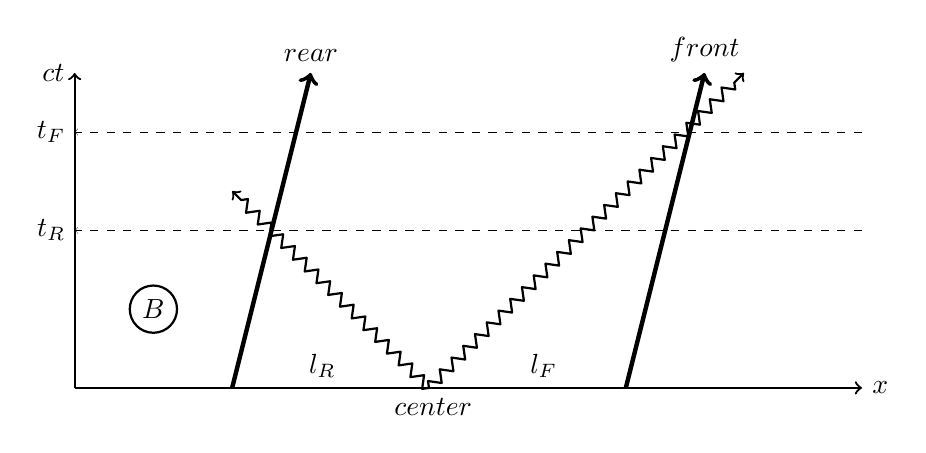
\begin{tikzpicture}[->, thick]
 	\draw (0,0,0) -- (0,4,0) node[left] {$ct$}; %+Y
 	\draw [ultra thick](2,0,0) -- (3,4,0) node[above] {$rear$}; %+y'
 	\draw [ultra thick](7,0,0) -- (8,4,0) node[above] {$front$}; %+y'
 	
 	\draw (0,0,0) -- (10,0,0) node[right] {$x$} node[above, xshift=-195] {$l_{R}$} node[above, xshift=-115]{$l_{F}$} node[below, xshift=-155]{$center$}; %+x
 	
 	\draw [dashed, ultra thin] (10,2) -- (0,2) node[left]{$t_{R}$}; %+x---
 	\draw [dashed, ultra thin] (10,3.25) -- (0,3.25) node[left]{$t_{F}$}; %+x---
 	
 	% light arrows
 	\draw [->, line join=round, decorate, decoration={zigzag, segment length=6, amplitude=2,post=lineto, post length=2pt}] (4.5,0) -- (2,2.5);
 	\draw [->, line join=round, decorate, decoration={zigzag, segment length=6, amplitude=2,post=lineto, post length=2pt}] (4.5,0) -- (8.5,4);
 	
 	%Bob's name:
 	\draw (1,1) circle [radius=0.3] node {$B$};
 	
 	\end{tikzpicture}
 	\caption{Bob's spacetime diagram, revisited}
 	\label{fig: bob's spacetime 4}
 \end{figure} 
 
 \noindent We often define the scaling so that light paths (wavy lines) make a 45-degree angle with the horizontal axis. Because no massive physical object can exceed the speed of light, particle paths are always more vertical than light paths.
 
 \noindent Mathematically, the speed of the particle relates to the slope of its path by:
 \begin{equation}
 \beta=\frac{u}{c}=\frac{\Delta x}{c\Delta t}=\frac{\Delta x}{\Delta (ct)}=\frac{1}{slope}.
 \end{equation}
 Therefore the slope magnitude of the object's path in spacetime must always be greater than 1 at any given point. 
 
 \noindent Minkowski (spacetime) diagram conventionally has a light-line intersecting the origin, as shown in Figure 29:
  \begin{figure}[!htb] %place figure here
 	\centering
 	\begin{tikzpicture}[->]
 	\draw [thick](0,0) -- (0,3) node[left] {$ct$} coordinate (ct); %+Y
 	%\draw [thick](0,0) -- (1.5,5.2) node[left] {$ct'$} coordinate (x); %+y'
 	%\draw [thick](0,0) -- (5.2,1.5) node[right] {$x'$} coordinate (x'); %+y'
 	\draw [thick](0,0) -- (3,0) node[right] {$x$} coordinate (ct'); 
 	
 	%\draw (5.5,0) coordinate (x) -- (0,0) coordinate (o) -- (5.2,1.5) coordinate (x') pic[draw=black, <->, angle eccentricity=2, angle radius=1.5cm] 
 	%{angle=x--o--x'};
 	
 	%\draw (0,5.5) coordinate (ct) -- (0,0) coordinate (o) -- (1.5,5.2) coordinate (ct') pic[draw=black, <->, angle eccentricity=2, angle radius=1.5cm]
 	%{angle=ct'--o--ct};
 	
 	%	node[above, xshift=-195] {$l_{R}$} 
 	%	node[above, xshift=-115]{$l_{F}$} 
 	%	node[below, xshift=-155]{$center$}; %+x
 	
 	%	\draw [dashed, ultra thin] (10,2) -- (0,2) 
 	%	node[left]{$t_{R}$}; %+x---
 	%	\draw [dashed, ultra thin] (10,3.25) -- (0,3.25) 
 	%	node[left]{$t_{F}$}; %+x---
 	
 	% light arrows
 	%	\draw [->, line join=round, decorate, decoration={zigzag, segment length=6, amplitude=2,post=lineto, post length=2pt}] (4.5,0) -- (2,2.5);
 	\draw [->, line join=round, decorate, decoration={zigzag, segment length=6, amplitude=1.5,post=lineto, post length=2pt}] (0,0) -- (2.75,2.75);
 	
 	%Bob's name:
 	%	\draw (1,1) circle [radius=0.3] node {$B$};
 	
 	% Angle
 	%\node at (2.75,0.27) {$\phi = \tan[-1](\beta)$};
 	%\node at (0.4,2.75) [rotate = 80] {$\phi = \tan[-1](\beta)$};
 	
 	\end{tikzpicture}
 	\caption{$(S')$, traveling at speed $v$ relative to $(S)$, represented in $(S)$.}
 	\label{Minkowski diagram}
 \end{figure}

 \subsubsection{Light-cones}
 Figure 30 shows a 2-dimensional projection of a light-cone onto a spacetime diagram. It is quite straightforward how we can construct a light-cone in a spacetime diagram: crossing two light-lines, one representing a beam in the $+x$ direction and the other in the $-x$, together roughly at their mid-points. However, it is crucial that we understand what light-cones do and their significance in special relativity.
 
 \noindent Light-cones are a good graphical representation of how events evolve in spacetime. What do we mean by this? Well, if we define the intersection of the light-lines to be the ``present,'' then the region between the light-lines above the ``present'' point represents the ``future,'' and the region below represents the ``past.'' Why?
 
 \noindent As discussed in 7.1.1, because any physical object must never exceed the speed of light, its path in spacetime always has slope with magnitude greater than 1. Consequently, if we let any point on its path be the ``present'' point, then the rest of the object's path is confined within two regions defined by a light-cone centered at the chosen ``present'' point. It makes sense for us to call the upper region ``future'' and the lower region ``past'' simply because time flows upwards in a spacetime diagram.
 
 \begin{figure}[!htb] %place figure here
 	\centering
 	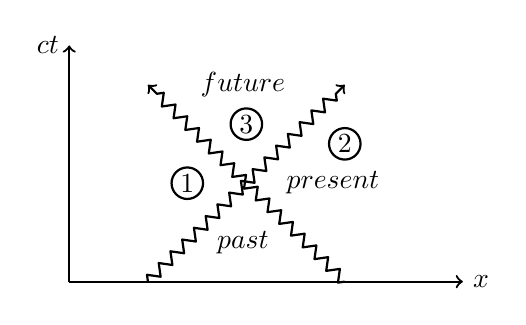
\begin{tikzpicture}[->, thick]
 	\draw (0,0,0) -- (0,3,0) node[left] {$ct$}; %+Y
 	
 	\draw (0,0,0) -- (5,0,0) 
 	node[right] {$x$} 
 	%node[above, xshift=-195] {$l_{R}$} 
 	%node[above, xshift=-115]{$l_{F}$} 
 	node[below, xshift=-1.1 in, yshift= 0.3 in]{$past$} 
 	node[below, xshift=-1.1 in, yshift= 1.1 in]{$future$}
 	node[below, xshift=-0.65 in, yshift= 0.6 in]{$present$}; %+x
 	
% 	\draw [dashed, ultra thin] (10,2) -- (0,2) 
%	node[left]{$t_{R}$}; %+x---
% 	\draw [dashed, ultra thin] (10,3.25) -- (0,3.25) 
%	node[left]{$t_{F}$}; %+x---
 	
 	% light arrows
 	\draw [->, line join=round, decorate, decoration={zigzag, segment length=6, amplitude=2,post=lineto, post length=2pt}] (3.5,0) -- (1,2.5);
 	\draw [->, line join=round, decorate, decoration={zigzag, segment length=6, amplitude=2,post=lineto, post length=2pt}] (1,0) -- (3.5,2.5);
 	
 	%Bob's name:
 	\draw (1.5,1.25) circle [radius=0.2] node {$1$};
 	\draw (3.5,1.75) circle [radius=0.2] node {$2$};
 	\draw (2.25,2) circle [radius=0.2] node {$3$};
 	
 	\end{tikzpicture}
 	\caption{An exemplary light-cone}
 	\label{An exemplary light-cone}
 \end{figure}

 \noindent The division of a spacetime diagram into different ``time domains'' allows us to categorize events into those that \underline{can} be causally related and those that \underline{cannot}. Let us define the first group as ``\textbf{time-like}'' events and the latter as ``\textbf{space-like}.''   
 
 \noindent Let Event 1 be the ``present'' point on our spacetime diagram. Consider Events 1 and 2:
 \begin{equation}
 \begin{split}
 \Delta x_{12}&=x_2-x_1 \\
 c\Delta t_{12}&=c(t_2-t_1)
 \end{split}
 \end{equation}
 \noindent We observe that $\Delta x_{12} > c\Delta t_{12}$, which means Events 1 and 2 are \underline{too far} apart that one event cannot trigger another without breaking the speed of light limit. In other words, Events 1 and 2 cannot be causally related, or they are ``space-like separated.'' Note that Event 2 is not in the light-cone.
 
 \noindent Consider Events 1 and 3:
 \begin{equation}
 \begin{split}
 \Delta x_{13}&=x_3-x_1\\
 c\Delta t_{13}&=c(t_3-t_1)
 \end{split}
 \end{equation} 
 \noindent Because $\Delta x_{13} < c\Delta t_{13}$, a subluminal signal can trigger one event after the other. In other words, Events 1 and 3 can be causally related, or they are ``time-like separated.'' Note that Event 3 is in the light-cone.
 
 
 \subsubsection{The $S'$ axes}
 Now we will study how to represent another moving frame $(S')$ with axes $ct'$ and $x'$ on a spacetime diagram of a rest frame $(S)$.
 \begin{figure}[!htb] %place figure here
	\centering
	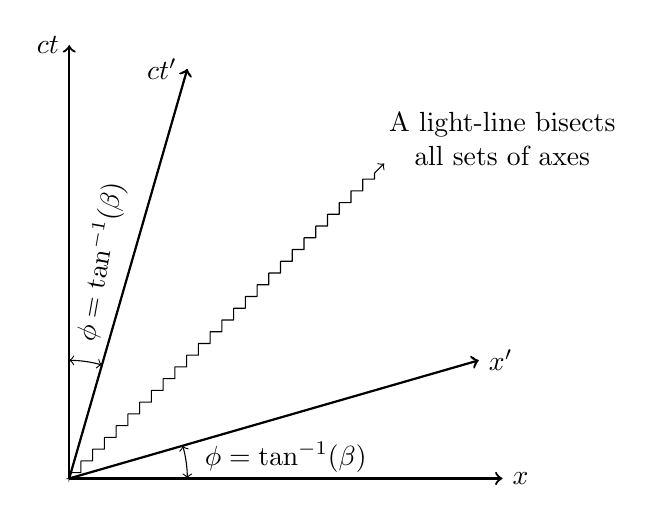
\begin{tikzpicture}[->]
	\draw [thick](0,0) -- (0,5.5) node[left] {$ct$}; %+Y
	\draw [thick](0,0) -- (1.5,5.2) node[left] {$ct'$}; %+y'
	\draw [thick](0,0) -- (5.2,1.5) node[right] {$x'$}; %+y'
	\draw [thick](0,0) -- (5.5,0) node[right] {$x$}; 
	
	\draw (5.5,0) coordinate (x) -- (0,0) coordinate (o) -- (5.2,1.5) coordinate (x') pic[draw=black, <->, angle eccentricity=2, angle radius=1.5cm]
	{angle=x--o--x'};
	
	\draw (0,5.5) coordinate (ct) -- (0,0) coordinate (o) -- (1.5,5.2) coordinate (ct') pic[draw=black, <->, angle eccentricity=2, angle radius=1.5cm]
	{angle=ct'--o--ct};
	
%	node[above, xshift=-195] {$l_{R}$} 
%	node[above, xshift=-115]{$l_{F}$} 
%	node[below, xshift=-155]{$center$}; %+x
	
%	\draw [dashed, ultra thin] (10,2) -- (0,2) 
%	node[left]{$t_{R}$}; %+x---
%	\draw [dashed, ultra thin] (10,3.25) -- (0,3.25) 
%	node[left]{$t_{F}$}; %+x---
	
	% light arrows
%	\draw [->, line join=round, decorate, decoration={zigzag, segment length=6, amplitude=2,post=lineto, post length=2pt}] (4.5,0) -- (2,2.5);
	
	%light-line
	\draw [->, line join=round, decorate, decoration={zigzag, segment length=6, amplitude=1.5,post=lineto, post length=2pt}] (0,0) -- (4,4);
	\node at (5.5,4.5) {A light-line bisects};
	\node at (5.5,4.1) {all sets of axes};
	
	%Bob's name:
%	\draw (1,1) circle [radius=0.3] node {$B$};

	% Angle
	\node at (2.75,0.27) {$\phi = \tan[-1](\beta)$};
	\node at (0.4,2.75) [rotate = 80] {$\phi = \tan[-1](\beta)$};
	
	\end{tikzpicture}
	\caption{$(S')$, traveling at speed $v$ relative to $(S)$, represented in $(S)$.}
	\label{$(S')$, traveling at speed $v$ relative to $(S)$, represented in $(S)$.}
\end{figure}

\noindent Note that the transformation of coordinates between $(S)$ and $(S')$ aren't orthogonal because lengths (and time intervals) are not \textit{invariant} quantities in special relativity. To state more simply, the spacetime diagram representing $(S')$ is ``squeezed'' between the axes of $(S)$ and the light-line instead of rotated or reflected about some axis, effectively stretching (and/or compressing) along the light-line. So what (physically) explains this ``squeezing'' action? Let us answer this question using (1) a physical, more intuitive, reasoning and (2) the Lorentz-Einstein transformation equations. We will see how the latter is a more advantageous approach. 

\noindent (For readers with background in linear algebra: The ``squeezing action'' is nothing but a geometrical representation of the Lorentz-Einstein transformation matrix in one spatial dimension.)

\noindent \textbf{i. A physical explanation}

\noindent Consider an object at $x'=0$ in $(S')$, which is traveling at speed $v$ relative to $(S)$. Assuming that the object is at rest in $(S')$, the line $x'=0$ (or equivalently  $ct'$) is the object's path in the spacetime of $(S')$. In our rest frame $(S)$, the object's path in the spacetime of $(S)$ is tilted an angle $\phi$ from the vertical ($ct$) because the object is effectively traveling at speed $v$ in $(S)$. As discussed in 7.1.1, $\phi$ characterizes how fast an object travels by:
\begin{equation}
\phi=\tan^{-1}(\beta)=\tan^{-1}\left( \frac{v}{c}\right) 
\end{equation}  

\noindent What about the ``up-tilt'' of the $x'$ axis from $x$? This is where our ``physical explanation'' gets less intuitive, because in order to explain how an object at $ct'=0$ (in $(S')$, of course) can be represented in $(S)$, we have to take into account two fundamental effects of relativity, namely length contraction and loss of simultaneity. While a careful inspection can lead us to $\phi=\tan^{-1}(\beta)$, the Lorentz-Einstein equations are obviously a better set of tools for tackling this problem. 

\noindent \textbf{ii. The Lorentz-Einstein explanation}

\noindent For the $x'=0$ case:
\begin{equation}
\begin{split}
&x=\beta ct\\
\therefore{}& \frac{ct}{x}=\frac{1}{\beta}=\frac{1}{slope}\\
\therefore{}& \phi=\tan^{-1}(\beta).
\end{split}
\end{equation}

\noindent For the $ct'=0$ case:
\begin{equation}
\begin{split}
& ct'=0\\
\therefore{}& ct=\beta x\\
\therefore{}& \frac{x}{ct}=\frac{1}{\beta}=\frac{1}{slope}\\
\therefore{}& \phi=\tan^{-1}(\beta).
\end{split}
\end{equation}

\subsubsection{Calibrating Scales}

\begin{figure}[!htb] %place figure here
	\centering
	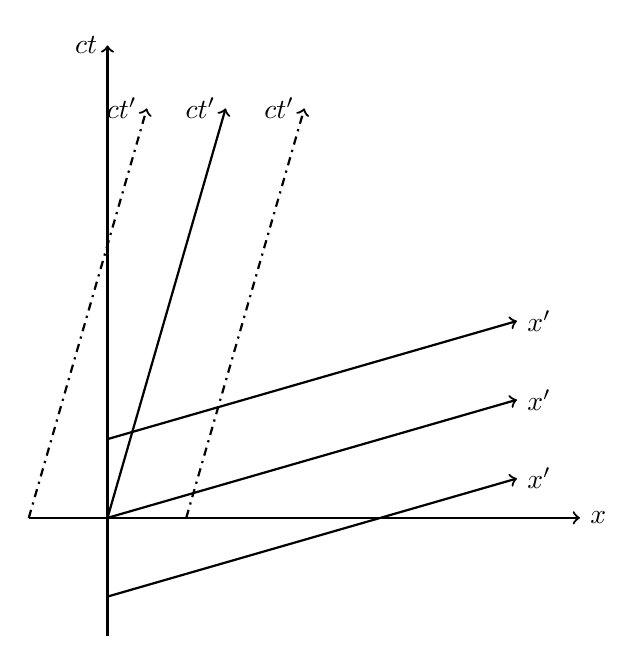
\begin{tikzpicture}[->]
	\draw [thick](0,-1.5) -- (0,6) node[left] {$ct$}; %+Y
	\draw [thick](0,0) -- (1.5,5.2) node[left] {$ct'$}; %+y'
	\draw [thick](0,0) -- (5.2,1.5) node[right] {$x'$}; %+y'
	\draw [thick](-1,0) -- (6,0) node[right] {$x$};
	\draw [thick](0,1) -- (5.2,2.5) node[right] {$x'$}; %+y'
	\draw [thick](0,-1) -- (5.2,0.5) node[right] {$x'$}; %+y' 
	\draw [thick, dash dot](-1,0) -- (0.5,5.2) node[left] {$ct'$}; %+y'
	\draw [thick, dash dot](1,0) -- (2.5,5.2) node[left] {$ct'$}; %+y'
	
	%\draw (5.5,0) coordinate (x) -- (0,0) coordinate (o) -- (5.2,1.5) coordinate (x') pic[draw=black, <->, angle eccentricity=2, angle radius=1.5cm]
	%{angle=x--o--x'};
	
	%\draw (0,5.5) coordinate (ct) -- (0,0) coordinate (o) -- (1.5,5.2) coordinate (ct') pic[draw=black, <->, angle eccentricity=2, angle radius=1.5cm]
	%{angle=ct'--o--ct};
	
	%	node[above, xshift=-195] {$l_{R}$} 
	%	node[above, xshift=-115]{$l_{F}$} 
	%	node[below, xshift=-155]{$center$}; %+x
	
	%	\draw [dashed, ultra thin] (10,2) -- (0,2) 
	%	node[left]{$t_{R}$}; %+x---
	%	\draw [dashed, ultra thin] (10,3.25) -- (0,3.25) 
	%	node[left]{$t_{F}$}; %+x---
	
	% light arrows
	%	\draw [->, line join=round, decorate, decoration={zigzag, segment length=6, amplitude=2,post=lineto, post length=2pt}] (4.5,0) -- (2,2.5);
	
	%light-line
	%\draw [->, line join=round, decorate, decoration={zigzag, segment length=6, amplitude=1.5,post=lineto, post length=2pt}] (0,0) -- (4,4);
	%\node at (5.5,4.5) {A light-line bisects};
	%\node at (5.5,4.1) {all sets of axes};
	
	%Bob's name:
	%	\draw (1,1) circle [radius=0.3] node {$B$};
	
	% Angle
	%\node at (2.75,0.27) {$\phi = \tan[-1](\beta)$};
	%\node at (0.4,2.75) [rotate = 80] {$\phi = \tan[-1](\beta)$};
	
	\end{tikzpicture}
	\caption{$(S')$, traveling at speed $v$ relative to $(S)$, represented in $(S)$.}
	\label{$(S')$, traveling at speed $v$ relative to $(S)$, represented in $(S)$ 1}
\end{figure}

\noindent Now we will demonstrate how ``lengths'' in the spacetime diagram of $(S')$ relate to ``lengths'' in the spacetime diagram of $(S)$. Consider the point ($x_0, 0$) in $(S')$. In $(S')$, the distance between this point and the origin is:
\begin{equation}
r'=\sqrt{{x_0}^2 + 0^2}={x_0}^2
\end{equation}
\noindent The question is ``In $(S')$, what is the distance between this point and the origin?'' To answer this we first find the $x$ and $ct$ components of this segment in $(S)$. The ``$x$'' component of the line segment:
\begin{equation}
\begin{split}
x&=\gamma(x'+\beta ct')\\
&=\gamma x' \\
&= \gamma x_0
\end{split}
\end{equation}
\noindent The ``$ct$'' component of the line segment:
\begin{equation}
\begin{split}
ct&=\gamma(ct'+\beta x')\\
&=\gamma\beta x_0
\end{split}
\end{equation}
\noindent Hence the length of the line segment in $(S)$, by Pythagorean theorem, is:
\begin{equation}
\begin{split}
r&=x_0\sqrt{\gamma^2 + (\gamma\beta)^2} \\
&=x_0\sqrt{\gamma^2(1+\beta^2)} \\
&=x_0\sqrt{\frac{1+\beta^2}{1-\beta^2}} \\
&=r'\sqrt{\frac{1+\beta^2}{1-\beta^2}} > 1
\end{split}
\end{equation}
We conclude that intervals in $(S')$ spacetime diagrams is stretched by $(1+\beta^2)/(1-\beta^2)$ as we move to $(S)$.
 
 \subsubsection{Causality and Minkowski diagrams}
 \noindent In 7.1.2 we briefly discussed ``time-like'' and ``space-like'' separated events. In this sectio we revisit these concepts in a more graphical sense through Minkowski spacetime diagrams.
 
 \noindent Consider two pairs of events: (1,2) and (3,4) in $(S)$. 
  \begin{figure}[!htb] %place figure here
 	\centering
 	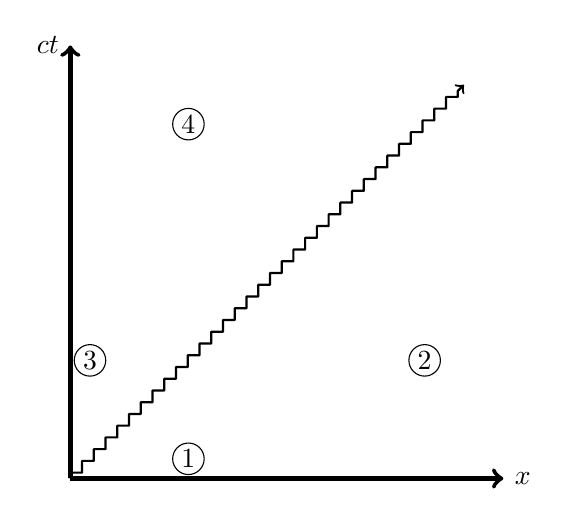
\begin{tikzpicture}[->]
 	\draw [ultra thick](0,0) -- (0,5.5) node[left] {$ct$}; %+Y
 	%\draw [thick](0,0) -- (1.5,5.2) node[left] {$ct'$}; %+y'
 	%\draw [thick](0,0) -- (5.2,1.5) node[right] {$x'$}; %+y'
 	\draw [ultra thick](0,0) -- (5.5,0) node[right] {$x$}; 
 	%\draw [thick, dashed](0,0) -- (3,5) node[left] {$ct''$}; %+y'
 	%\draw [thick, dashed](0,0) -- (5,3) node[right] {$x''$}; %+y'
 	
 	%\draw (5.5,0) coordinate (x) -- (0,0) coordinate (o) -- (5.2,1.5) coordinate (x') pic[draw=black, <->, angle eccentricity=2, angle radius=1.5cm]
 	%{angle=x--o--x'};
 	
 	%\draw (0,5.5) coordinate (ct) -- (0,0) coordinate (o) -- (1.5,5.2) coordinate (ct') pic[draw=black, <->, angle eccentricity=2, angle radius=1.5cm]
 	%{angle=ct'--o--ct};
 	
 	%	node[above, xshift=-195] {$l_{R}$} 
 	%	node[above, xshift=-115]{$l_{F}$} 
 	%	node[below, xshift=-155]{$center$}; %+x
 	
 	%	\draw [dashed, ultra thin] (10,2) -- (0,2) 
 	%	node[left]{$t_{R}$}; %+x---
 	%	\draw [dashed, ultra thin] (10,3.25) -- (0,3.25) 
 	%	node[left]{$t_{F}$}; %+x---
 	
 	% light arrows
 	%	\draw [->, line join=round, decorate, decoration={zigzag, segment length=6, amplitude=2,post=lineto, post length=2pt}] (4.5,0) -- (2,2.5);
 	
 	%light-line
 	\draw [->, thick, line join=round, decorate, decoration={zigzag, segment length=6, amplitude=1.5,post=lineto, post length=2pt}] (0,0) -- (5,5);
 	%\node at (5.5,4.5) {A light-line bisects};
 	%\node at (5.5,4.1) {all sets of axes};
 	
 	%Bob's name:
 	%	\draw (1,1) circle [radius=0.3] node {$B$};
 	
 	% Angle
 	%\node at (2.75,0.27) {$\phi = \tan[-1](\beta)$};
 	%\node at (0.4,2.75) [rotate = 80] {$\phi = \tan[-1](\beta)$};
 	
 	\draw (1.5,0.25) circle [radius=0.2] node {$1$};
 	\draw (4.5,1.5) circle [radius=0.2] node {$2$};
 	\draw (0.25,1.5) circle [radius=0.2] node {$3$};
 	\draw (1.5,4.5) circle [radius=0.2] node {$4$};
 	
 	\end{tikzpicture}
 	\caption{$(S')$, traveling at speed $v$ relative to $(S)$, represented in $(S)$.}
 	\label{$(S')$, traveling at speed $v$ relative to $(S)$, represented in $(S)$ 3}
 \end{figure}

\noindent Consider the first pair, (1,2). There exists a frame, say $(S')$ in which 1 and 2 are simultaneous. There also exists a frame, say $(S'')$, in which the chronological order of these two events is reversed: 
\begin{figure}[!htb] %place figure here
	\centering
	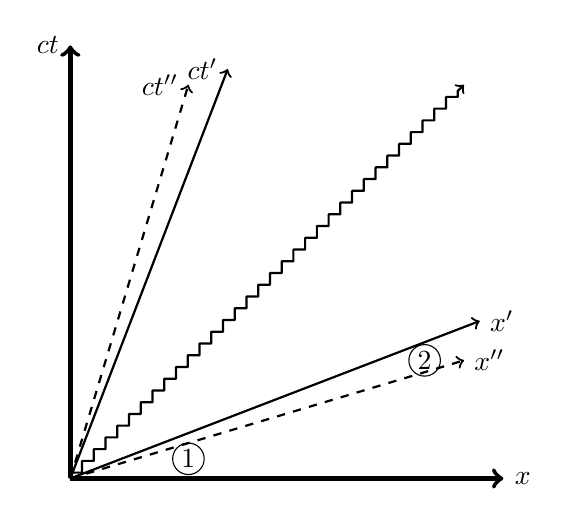
\begin{tikzpicture}[->]
	\draw [ultra thick](0,0) -- (0,5.5) node[left] {$ct$}; %+Y
	\draw [thick](0,0) -- (2,5.2) node[left] {$ct'$}; %+y'
	\draw [thick](0,0) -- (5.2,2) node[right] {$x'$}; %+y'
	\draw [ultra thick](0,0) -- (5.5,0) node[right] {$x$}; 
	\draw [thick, dashed](0,0) -- (1.5,5) node[left] {$ct''$}; %+y'
	\draw [thick, dashed](0,0) -- (5,1.5) node[right] {$x''$}; %+y'
	
	%\draw (5.5,0) coordinate (x) -- (0,0) coordinate (o) -- (5.2,1.5) coordinate (x') pic[draw=black, <->, angle eccentricity=2, angle radius=1.5cm]
	%{angle=x--o--x'};
	
	%\draw (0,5.5) coordinate (ct) -- (0,0) coordinate (o) -- (1.5,5.2) coordinate (ct') pic[draw=black, <->, angle eccentricity=2, angle radius=1.5cm]
	%{angle=ct'--o--ct};
	
	%	node[above, xshift=-195] {$l_{R}$} 
	%	node[above, xshift=-115]{$l_{F}$} 
	%	node[below, xshift=-155]{$center$}; %+x
	
	%	\draw [dashed, ultra thin] (10,2) -- (0,2) 
	%	node[left]{$t_{R}$}; %+x---
	%	\draw [dashed, ultra thin] (10,3.25) -- (0,3.25) 
	%	node[left]{$t_{F}$}; %+x---
	
	% light arrows
	%	\draw [->, line join=round, decorate, decoration={zigzag, segment length=6, amplitude=2,post=lineto, post length=2pt}] (4.5,0) -- (2,2.5);
	
	%light-line
	\draw [->, thick, line join=round, decorate, decoration={zigzag, segment length=6, amplitude=1.5,post=lineto, post length=2pt}] (0,0) -- (5,5);
	%\node at (5.5,4.5) {A light-line bisects};
	%\node at (5.5,4.1) {all sets of axes};
	
	%Bob's name:
	%	\draw (1,1) circle [radius=0.3] node {$B$};
	
	% Angle
	%\node at (2.75,0.27) {$\phi = \tan[-1](\beta)$};
	%\node at (0.4,2.75) [rotate = 80] {$\phi = \tan[-1](\beta)$};
	
	\draw (1.5,0.25) circle [radius=0.2] node {$1$};
	\draw (4.5,1.5) circle [radius=0.2] node {$2$};
	%\draw (1,2.2) circle [radius=0.2] node {$3$};
	%\draw (2,4) circle [radius=0.2] node {$4$};
	
	\end{tikzpicture}
	\caption{$(S')$, traveling at speed $v$ relative to $(S)$, represented in $(S)$.}
	\label{$(S')$, traveling at speed $v$ relative to $(S)$, represented in $(S)$ 4}
\end{figure}

\noindent Events 1 and 2 cannot be causally related (since their chronological order can be reversed). We say events 1 and 2 are ``space-like separated.''

\noindent Similarly, consider the second pair of events, (3,4). There exists a frame, say $(S')$ in which 3 and 4 are at the same location. However, the chronological order of events 3 and 4 cannot be reversed.  
\begin{figure}[!htb] %place figure here
	\centering
	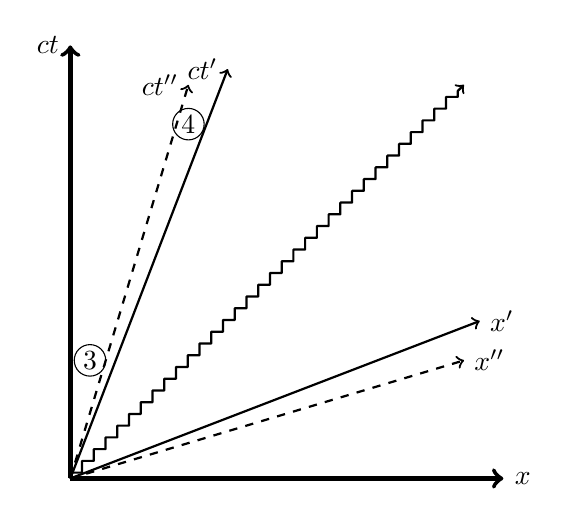
\begin{tikzpicture}[->]
	\draw [ultra thick](0,0) -- (0,5.5) node[left] {$ct$}; %+Y
	\draw [thick](0,0) -- (2,5.2) node[left] {$ct'$}; %+y'
	\draw [thick](0,0) -- (5.2,2) node[right] {$x'$}; %+y'
	\draw [ultra thick](0,0) -- (5.5,0) node[right] {$x$}; 
	\draw [thick, dashed](0,0) -- (1.5,5) node[left] {$ct''$}; %+y'
	\draw [thick, dashed](0,0) -- (5,1.5) node[right] {$x''$}; %+y'
	
	%\draw (5.5,0) coordinate (x) -- (0,0) coordinate (o) -- (5.2,1.5) coordinate (x') pic[draw=black, <->, angle eccentricity=2, angle radius=1.5cm]
	%{angle=x--o--x'};
	
	%\draw (0,5.5) coordinate (ct) -- (0,0) coordinate (o) -- (1.5,5.2) coordinate (ct') pic[draw=black, <->, angle eccentricity=2, angle radius=1.5cm]
	%{angle=ct'--o--ct};
	
	%	node[above, xshift=-195] {$l_{R}$} 
	%	node[above, xshift=-115]{$l_{F}$} 
	%	node[below, xshift=-155]{$center$}; %+x
	
	%	\draw [dashed, ultra thin] (10,2) -- (0,2) 
	%	node[left]{$t_{R}$}; %+x---
	%	\draw [dashed, ultra thin] (10,3.25) -- (0,3.25) 
	%	node[left]{$t_{F}$}; %+x---
	
	% light arrows
	%	\draw [->, line join=round, decorate, decoration={zigzag, segment length=6, amplitude=2,post=lineto, post length=2pt}] (4.5,0) -- (2,2.5);
	
	%light-line
	\draw [->, thick, line join=round, decorate, decoration={zigzag, segment length=6, amplitude=1.5,post=lineto, post length=2pt}] (0,0) -- (5,5);
	%\node at (5.5,4.5) {A light-line bisects};
	%\node at (5.5,4.1) {all sets of axes};
	
	%Bob's name:
	%	\draw (1,1) circle [radius=0.3] node {$B$};
	
	% Angle
	%\node at (2.75,0.27) {$\phi = \tan[-1](\beta)$};
	%\node at (0.4,2.75) [rotate = 80] {$\phi = \tan[-1](\beta)$};
	
	%\draw (1.5,0.25) circle [radius=0.2] node {$1$};
	%\draw (4.5,1.5) circle [radius=0.2] node {$2$};
	\draw (0.25,1.5) circle [radius=0.2] node {$3$};
	\draw (1.5,4.5) circle [radius=0.2] node {$4$};
	
	\end{tikzpicture}
	\caption{$(S')$, traveling at speed $v$ relative to $(S)$, represented in $(S)$.}
	\label{$(S')$, traveling at speed $v$ relative to $(S)$, represented in $(S)$ 5}
\end{figure}

\noindent Events 3 and 4 can be causally related (since their chronological order cannot be reversed). We say events 3 and 4 are ``time-like separated.''

 
 \subsection{How does Relativity explain Stellar Aberration?}
 
 \subsection{The Space-Time interval: An \textit{Invariant}}
 Is there a quantity that uniquely and, in a frame-independent way, identifies the ``kind'' of separation between events? The answer is yes, and this quantity is called ``spacetime interval,'' defined mathematically as:
 \begin{equation}
 (\Delta S)^2=(c\Delta t)^2-(\Delta x)^2 - (\Delta y)^2 - (\Delta z)^2.
 \end{equation}
 Note that this quantity is a scalar. We can in fact show, quite quickly, that this quantity is frame-independent. Consider a narrow case with two frames $(S)$ and $(S')$, where $(S')$ is traveling at speed $v$ in the $x$-direction relative to $(S)$. We will show $(\Delta S)^2 = (\Delta S')^2$, using the Lorentz-Einstein transformation equations:
 \begin{equation}
 \begin{split}
 (\Delta S')^2&=(c\Delta t')^2-(\Delta x')^2-(\Delta y')^2-(\Delta z')^2 \\
 &=\gamma^2(c\Delta t-\beta \Delta x)^2-\gamma^2(\Delta x - \beta c\Delta t)^2-(\Delta y')^2-(\Delta z')^2 \\ 
 &=\gamma^2((c\Delta t)^2-2c\Delta t\beta \Delta x+(\beta \Delta x)^2)-\gamma^2((\Delta x)^2 -2\beta c\Delta t \Delta x + (\beta c\Delta t)^2)\\&-(\Delta y')^2-(\Delta z')^2 \\
 &=(\Delta t)^2(\gamma^2 c^2 - \gamma^2 v^2)+(\Delta x)^2(\gamma^2\beta^2 - \gamma^2)-(\Delta y')^2-(\Delta z')^2\\
 &= (c\Delta t)^2(1-\beta^2)-(\Delta x)^2(1-\beta^2)\gamma^2-(\Delta y')^2-(\Delta z')^2
 \end{split}
 \end{equation}
 Now, since $\gamma^2=1/(1-\beta^2)$, $\Delta y = \Delta y'$, and $\Delta x' = \Delta x$, we obtain the following:
 \begin{equation}
 (\Delta S')^2=(c\Delta t)^2-(\Delta x)^2-(\Delta y)^2-(\Delta z)^2 = (\Delta S)^2
 \end{equation}
 
 Now we 
 \subsection{The Twin Paradox}
 \subsubsection{Einstein's clock paradox}
 \subsubsection{Elapsed proper time}
 
 \newpage
 
 \section{Four-vectors}
 \subsection{Three-vectors}
 \subsubsection{The power of vector notations}
 \subsubsection{The prototype vector}
 \subsubsection{What is a 3-vector?}
 \subsubsection{What is a scalar?}
 \subsubsection{Combination of vectors and scalar?}
 
 \subsection{Four-vectors}
 \subsubsection{The power of 4-vector notation}
 \subsubsection{The prototype 4-vector}
 \subsubsection{What is a 4-vector?}
 \subsubsection{Combination of 4-vectors and 4-scalars}
 
 \subsection{Four-velocity}
 \subsubsection{Four-velocity transformation}
 \subsubsection{The meaning of \underline{u}}
 
 \subsection{Four-acceleration}
  \newpage
 \section{Relativistic Dynamics}
 \subsection{Classical mechanics}
 hi
 \subsection{Four-momentum}
 hi
 \subsection{Interpretation of four-momentum}
  hi
  \subsubsection{Non-relativistic reduction}
  hi
  \subsubsection{Interpretation of $P_{0}$ and $\vec{P}$}
  hi
  \subsubsection{The equivalence of mass and energy}
  hi
  \subsubsection{Relativistic kinetic energy}
  hi
  \subsubsection{The energy-momentum invariant}
  hi
  \subsubsection{The energy-momentum transformation}
  hi
 
 \subsection{Testing four-momentum conservation}
 \subsubsection{Relativistic billiard problem}
 \paragraph{i) Newtonian mechanics results}
 \paragraph{ii) Relativistic results}
 \subsubsection{Collisions and Particle Creation}
 
 \subsection{Forces and relativistic dynamics}
 \subsubsection{Acceleration, velocity, mass}
 \subsubsection{The four-force}
 
  \newpage
 
 \section{The General Theory of Relativity - A brief introduction}
 - Special Relativity considers observers in inertial frames.\\
 - General Relativity observations in relativity accelerating frames. This is the theory of gravity!
 
 \subsection{Why Einstein included gravity in theory of General Relativity}
 \subsubsection{Newton's gravitation}
 \subsubsection{Problems with Newton's gravitation}
 
 \subsection{The Equivalence Principle}
 - In a truly falling frame, you \underline{do} eliminate gravity. Hence, the rules of special relativity hold.\\ 
 - There is NO observable difference between a real acceleration and gravity.\\ 
 - The ``strong'' equivalence principle:
 In a freely falling frame, all of the law  of physics obey the rules of special relativity. 
 \subsubsection{Freely falling light}
 Light's path in a gravitational field is curved.
 \subsubsection{Gravitational time dilation: Gravitational Redshift}
 
 
\end{document}
